\documentclass[12pt, a4paper]{article}
\usepackage{ctex}
\usepackage{geometry}
\usepackage{graphicx}
\usepackage{booktabs}
\usepackage{listings}
\usepackage{longtable}
\usepackage{multirow}
\usepackage{makecell}
\usepackage{tabularx}
\usepackage{amssymb}
\usepackage{setspace}
\usepackage{tabularx}
\usepackage{amssymb}  
\usepackage{float}

\geometry{left=2.5cm, right=2.5cm, top=3cm, bottom=3cm}
\setlength{\parskip}{0.5em}
\linespread{1.2}

\title{\textbf{\Large 图书管理系统 详细设计}}
\author{}
\date{}

\begin{document}
\newpage
\maketitle
\newpage
\tableofcontents
\newpage

\section{引言}

\subsection{文档目的}

本文档为图书管理系统的详细设计说明书，基于需求分析文档完成全维度设计落地，明确系统的架构分层、模块职责、接口规范、类结构等核心内容，为系统提供标准化、可落地的技术指导，同时确保系统设计符合软件工程行业规范与高内聚、低耦合的设计原则。

\subsection{适用范围}

本文档适用于图书管理系统的全生命周期，对应系统核心模块包括：认证授权模块、图书管理模块、借阅管理模块、系统管理模块，不包含需求文档明确不支持的借阅期限、逾期处罚、图书预约功能。

\subsection{名词定义}

\begin{table}[H]
    \centering
    \begin{tabular}{|l|l|}
        \hline
        名词 & 定义与说明 \\
        \hline
        ISBN & 国际标准书号，图书的唯一业务标识符 \\
        \hline
        借阅记录 & 记录图书借阅人、借阅时间、归还时间、图书ISBN等核心信息的业务数据 \\
        \hline
        库存 & 图书当前可借阅的可用数量 \\
        \hline
        未归还 & 图书已借出但尚未完成归还操作的借阅记录状态 \\
        \hline
        Token & 用户登录成功后生成的唯一身份凭证，用于接口访问的身份校验 \\
        \hline
        DTO & 数据传输对象，用于模块间的数据交互载体 \\
        \hline
        DAO & 数据访问对象，封装本地存储的读写操作 \\
        \hline
    \end{tabular}
\end{table}

\newpage
\section{总体架构设计}

\subsection{分层架构设计}
系统遵循五层分层架构设计，严格遵循高内聚、低耦合的面向对象设计原则，各层职责边界清晰，单向依赖，架构图如下：
\vspace{2cm}
\begin{figure}[H]
    \centering
    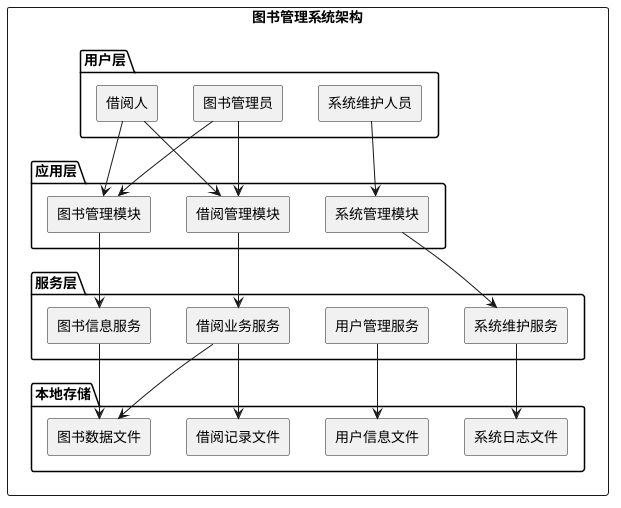
\includegraphics[width=0.8\textwidth]{ArchitctureDesignMod.png}
    \caption{图书管理系统架构图}
\end{figure}

\newpage
\begin{table}[H]
    \centering
    \begin{tabularx}{\linewidth}{|X|X|X|X|}
        \hline
        架构分层 & 层级职责 & 核心组件 & 依赖关系 \\
        \hline
        用户层 & 系统用户交互入口，负责发起业务操作请求 & 借阅人、图书管理员、系统维护人员 & 仅单向依赖应用层，无下层依赖 \\
        \hline
        应用层 & 接收用户请求，分发业务指令，封装前端业务流程，调度对应服务能力 & 图书管理模块、借阅管理模块、系统管理模块 & 单向依赖服务层，仅被用户层依赖 \\
        \hline
        服务层 & 封装系统核心业务逻辑，处理业务规则，为应用层提供标准化服务支撑 & 图书信息服务、借阅业务服务、用户管理服务、系统维护服务 & 单向依赖本地存储层，仅被应用层依赖 \\
        \hline
        本地存储层 & 负责系统全量数据的持久化存储与读写，屏蔽底层存储细节 & 图书数据文件、借阅记录文件、用户信息文件、系统日志文件 & 无底层依赖，被服务层单向依赖 \\
        \hline
    \end{tabularx}
\end{table}

\subsection{核心模块划分}

系统划分为4个核心功能模块，完整覆盖需求文档所有业务场景，模块职责如下：
\begin{enumerate}
    \item 认证授权模块：负责用户登录、身份校验、会话管理、权限控制，是系统的安全入口，包含用户登录、登出、Token校验等功能。

    \item 图书管理模块：负责图书信息的全生命周期管理，包括图书新增、查询、修改、删除、库存管理等功能。

    \item借阅管理模块：负责图书借阅、归还全流程处理，借阅记录的多维度查询与状态管理

    \item 系统管理模块：负责系统数据备份、数据恢复、系统配置管理，保障系统数据安全与稳定运行
\end{enumerate}

\newpage
\subsection{角色权限矩阵}

基于需求文档定义的三类核心用户，明确各角色的操作权限边界，如下：

\begin{table}[H]
    \centering
    \begin{tabularx}{\linewidth}{|X|X|c|c|c|}
        \hline
        功能模块 & 功能点 & 普通用户 & 图书管理员 & 系统维护人员 \\
        \hline
        认证授权模块 & 系统登录 & $\checkmark$ & $\checkmark$ & $\checkmark$ \\
        \hline
        & 登出系统 & $\checkmark$ & $\checkmark$ & $\checkmark$ \\
        \hline
        图书管理模块 & 图书多条件查询 & $\checkmark$ & $\checkmark$ & $\times$ \\
        \hline
        & 新增图书 & $\times$ & $\checkmark$ & $\times$ \\
        \hline
        & 修改图书信息 & $\times$ & $\checkmark$ & $\times$ \\
        \hline
        & 删除图书 & $\times$ & $\checkmark$ & $\times$ \\
        \hline
        借阅管理模块 & 图书借阅 & $\checkmark$ & $\checkmark$ & $\times$ \\
        \hline
        & 图书归还 & $\checkmark$ & $\checkmark$ & $\times$ \\
        \hline
        & 查看个人借阅记录 & $\checkmark$ & $\checkmark$ & $\times$ \\
        \hline
        & 查看所有借阅记录 & $\times$ & $\checkmark$ & $\times$ \\
        \hline
        & 查看未归还借阅记录 & $\times$ & $\checkmark$ & $\times$ \\
        \hline
        系统管理模块 & 数据备份 & $\times$ & $\times$ & $\checkmark$ \\
        \hline
        & 数据恢复 & $\times$ & $\times$ & $\checkmark$ \\
        \hline
        & 系统运行维护 & $\times$ & $\times$ & $\checkmark$ \\
        \hline
    \end{tabularx}
\end{table}

\newpage
\section{功能拆分与详细定义}

基于需求文档与模块划分，拆分为可落地的最小功能点，明确每个功能点的核心目标、前置条件、后置条件，如下：

\subsection{认证授权模块}

\begin{table}[H]
    \centering
    \begin{tabularx}{\linewidth}{|l|l|X|X|X|}
        \hline
        功能点编号 & 功能点名称 & 核心目标 & 前置条件 & 后置条件 \\
        \hline
        Auth-001 & 登录页面开发 & 实现标准化登录界面，支持用户名密码、验证码输入 & 前端工程搭建完成，可正常访问 & 页面可正常渲染，适配主流分辨率 \\
        \hline
        Auth-002 & 验证码生成接口 & 生成图形验证码，存入缓存，防止暴力登录 & 已集成验证码生成工具，缓存服务可用 & 验证码图片正常返回，缓存中存入对应验证码值，设置过期时间 \\
        \hline
        Auth-003 & 登录接口 & 完成用户身份校验，生成登录凭证 & 用户已访问登录页面，获取验证码与token & 校验通过生成Token，缓存用户登录信息，返回用户信息与权限；校验失败返回明确错误信息 \\
        \hline
        Auth-004 & 登录校验拦截器 & 实现所有业务接口的身份校验与权限控制 & 用户登录成功生成Token & 无Token/Token过期/权限不足的请求直接拦截，合法请求放行 \\
        \hline
        Auth-005 & 登出接口 & 清除用户登录状态，销毁Token & 用户已登录，持有有效Token & 缓存中删除用户登录信息，前端清除本地Token，返回登出成功 \\
        \hline
    \end{tabularx}
\end{table}

\newpage
\subsection{图书管理模块}

\begin{table}[H]
    \centering
    \begin{tabularx}{\linewidth}{|l|l|X|X|X|}
        \hline
        功能点编号 & 功能点名称 & 核心目标 & 前置条件 & 后置条件 \\
        \hline
        Book-001 & 图书多条件查询 & 支持按书名、作者、ISBN精准/模糊查询图书 & 用户已登录，拥有图书查询权限 & 返回匹配的图书列表，无匹配结果返回空列表与提示 \\
        \hline
        Book-002 & 图书新增 & 图书管理员录入图书信息，完成图书入库 & 用户已登录，拥有图书管理权限 & 校验通过后图书信息写入存储，库存同步更新，图书列表刷新 \\
        \hline
        Book-003 & 图书信息修改 & 编辑已入库图书的基础信息与库存 & 用户已登录，拥有图书管理权限，已定位目标图书 & 校验通过后更新存储中的图书信息，图书列表同步刷新最新数据 \\
        \hline
        Book-004 & 图书删除 & 下架并删除目标图书数据 & 用户已登录，拥有图书管理权限，已定位目标图书 & 校验无未归还借阅记录后，永久删除图书数据，图书列表同步更新 \\
        \hline
    \end{tabularx}
\end{table}

\subsection{借阅管理模块}

\begin{table}[H]
    \centering
    \begin{tabularx}{\linewidth}{|l|l|X|X|X|}
        \hline
        功能点编号 & 功能点名称 & 核心目标 & 前置条件 & 后置条件 \\
        \hline
        Borrow-001 & 图书借阅 & 完成图书借阅操作，扣减库存，生成借阅记录 & 用户已登录，目标图书存在且库存>0 & 生成借阅记录，状态标记为未归还，数据更新 \\
        \hline
        Borrow-002 & 图书归还 & 完成图书归还操作，恢复库存，更新借阅记录状态 & 用户已登录，存在对应未归还的有效借阅记录 & 借阅记录更新归还时间与已归还状态，数据更新 \\
        \hline
        Borrow-003 & 借阅记录多维度查询 & 支持按借阅人、借阅状态、时间范围查询借阅记录 & 用户已登录，拥有对应借阅记录查询权限 & 返回匹配的借阅记录列表，关联对应图书信息，无匹配结果返回提示 \\
        \hline
    \end{tabularx}
\end{table}

\subsection{系统管理模块}

\begin{table}[H]
    \centering
    \begin{tabularx}{\linewidth}{|l|l|X|X|X|}
        \hline
        功能点编号 & 功能点名称 & 核心目标 & 前置条件 & 后置条件 \\
        \hline
        System-001 & 数据备份 & 全量备份系统图书、借阅记录、用户数据 & 用户已登录，拥有系统维护权限 & 生成加密备份文件，记录备份时间与版本，返回备份结果 \\
        \hline
        System-002 & 数据恢复 & 基于备份文件恢复系统全量数据 & 用户已登录，拥有系统维护权限，备份文件有效 & 校验备份文件合法性后，恢复系统数据，记录恢复日志，返回恢复结果 \\
        \hline
    \end{tabularx}
\end{table}

\newpage
\section{核心用例图}
本核心用例图围绕图书管理系统的普通用户与图书管理员两类角色，完整呈现了图书借阅、归还、信息管理、记录查询等核心业务功能
\begin{figure}[H]
    \centering
    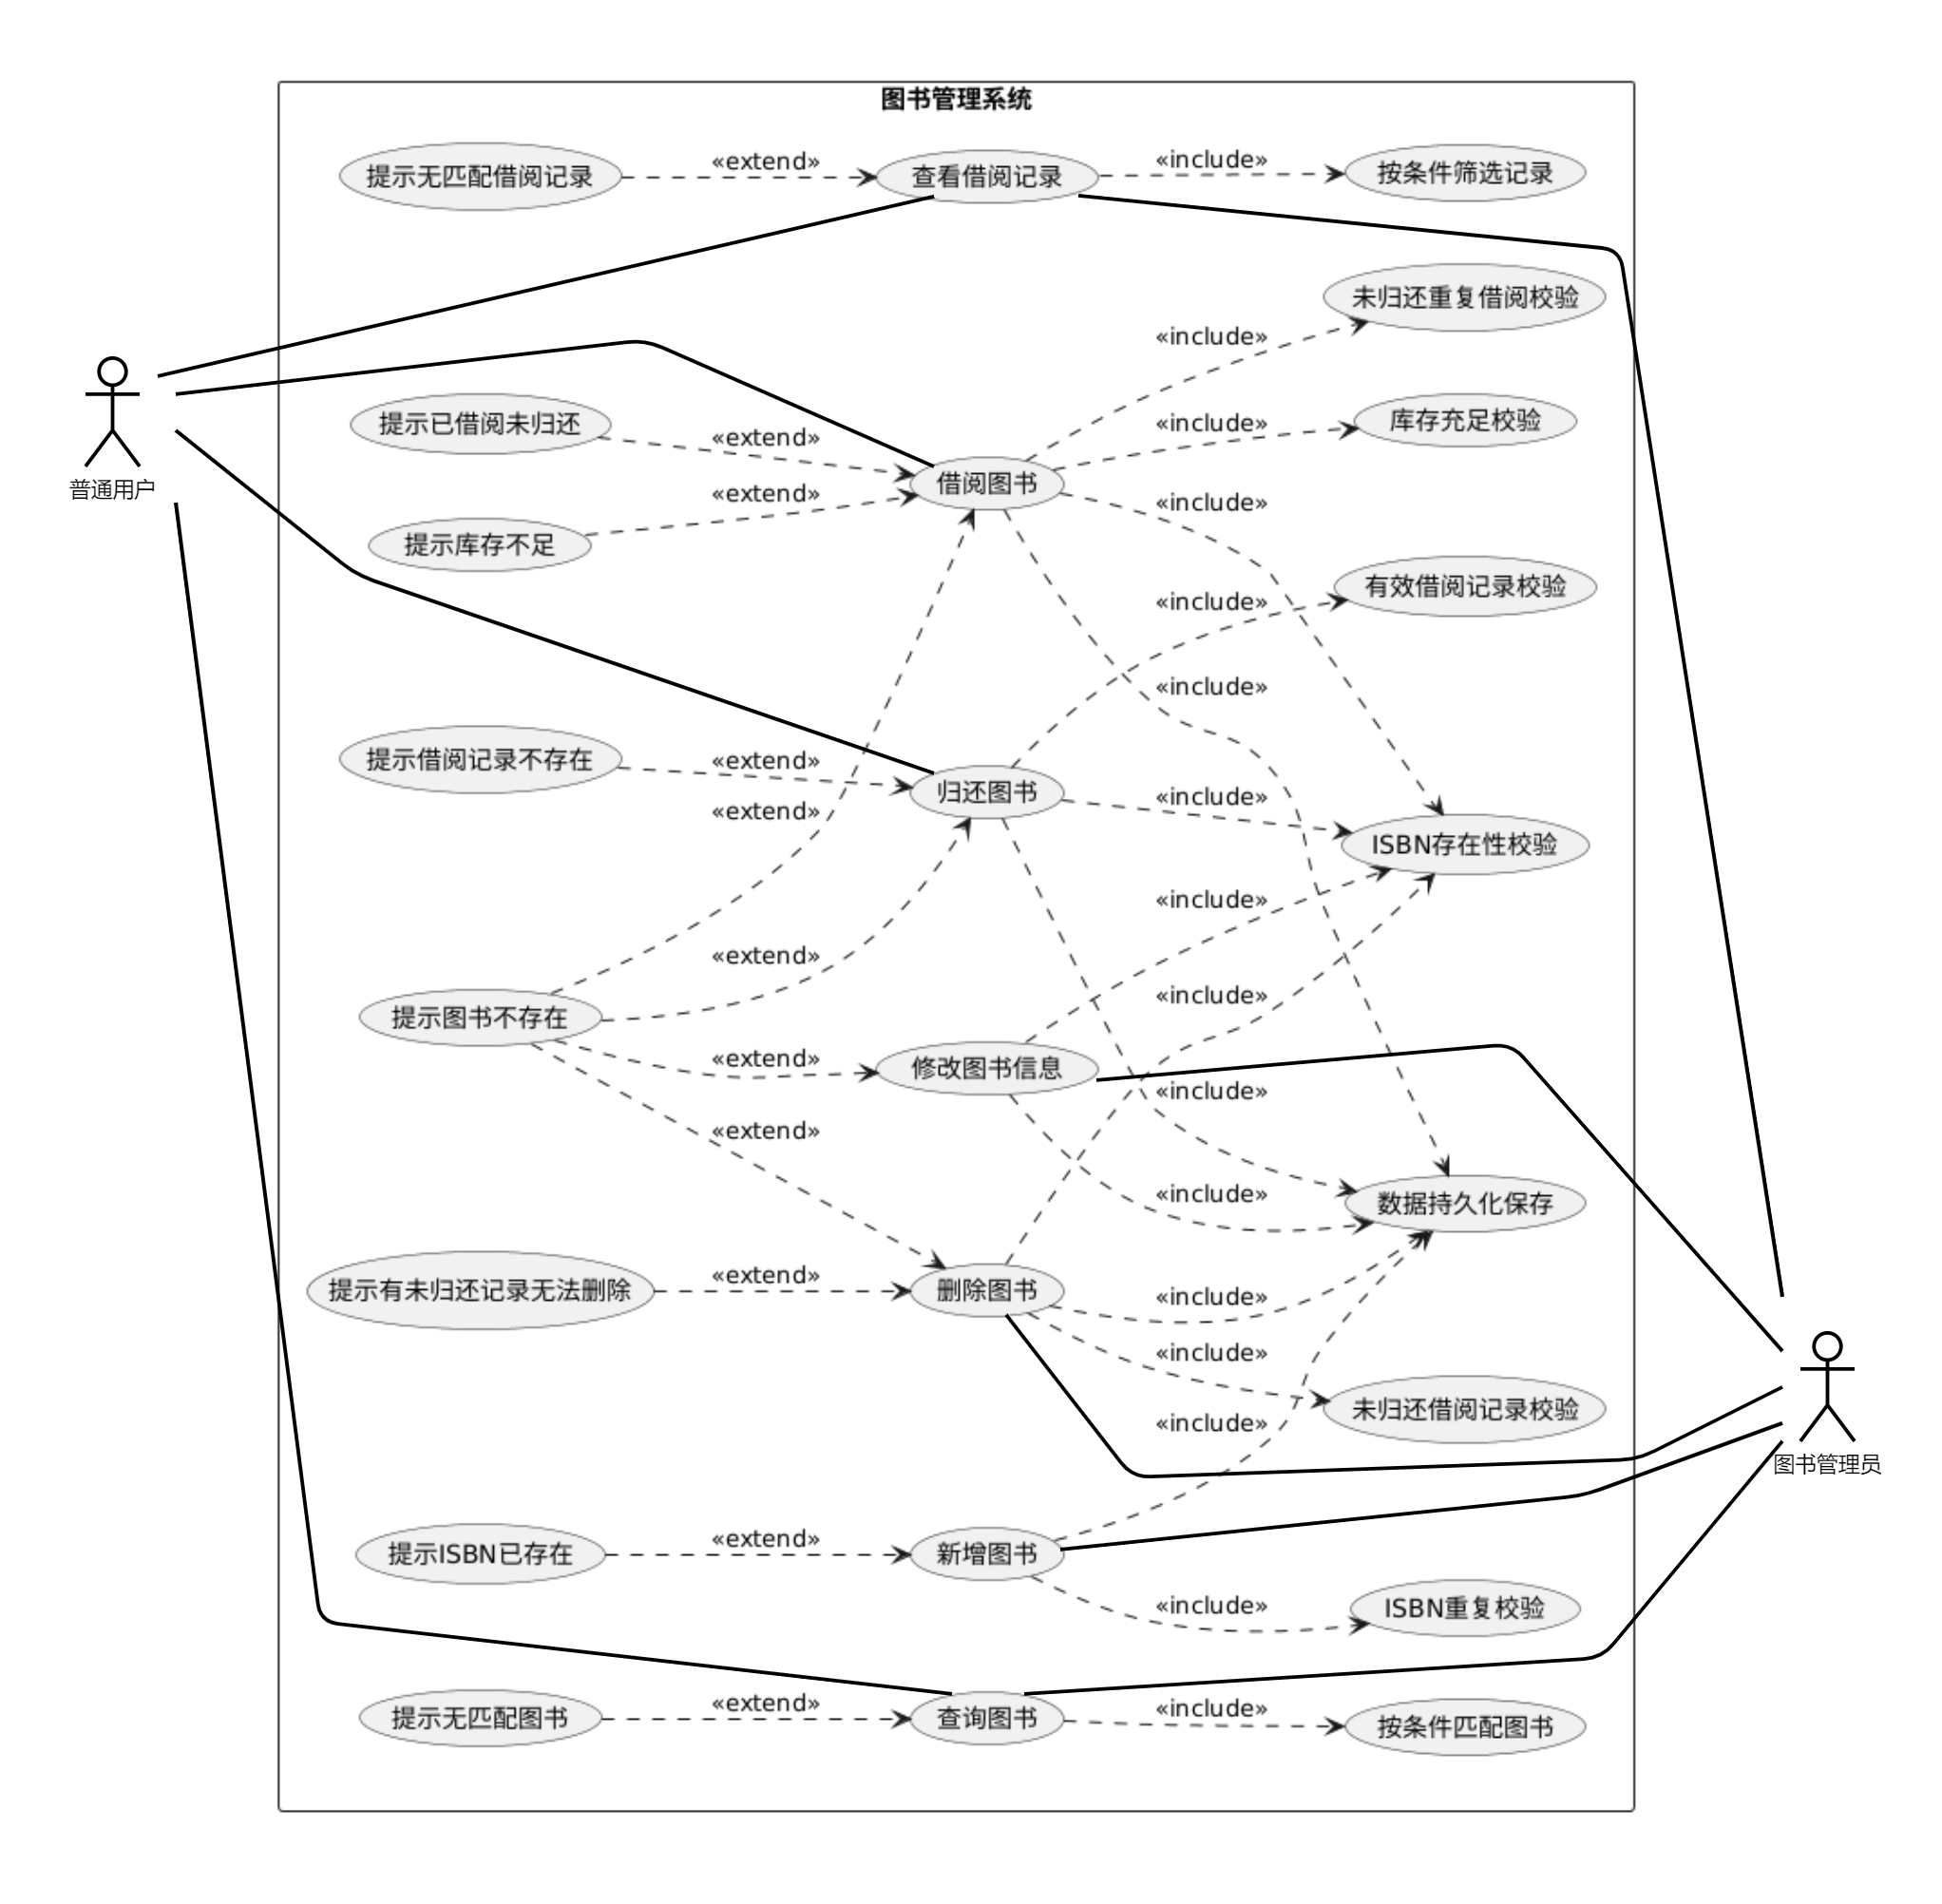
\includegraphics[width=0.8\textwidth]{DetailedUseCase.png}
    \caption{图书管理系统核心用例图}
\end{figure}


\newpage
\section{接口详细设计}

接口统一规范：

\begin{enumerate}
\item  基础请求路径：/api/v1

\item  统一响应格式：{"code": 状态码, "msg": 提示信息, "data": 响应数据}

\item  所有业务接口请求头必须携带Authorization: Bearer {Token}，由拦截器统一校验

\item  数据格式：JSON，字符编码：UTF-8
\end{enumerate}

\subsection{认证授权模块接口}

\subsubsection{验证码接口}



\begin{table}[H]
    \paragraph{接口信息}
    \centering
    \begin{tabular}{|l|l|}
        \hline
        项目 & 详情 \\
        \hline
        接口描述 & 生成图形验证码，返回验证码图片，同时将验证码值存入缓存 \\
        \hline
        接口地址 & /api/v1/auth/image-code/{imageCodeToken} \\
        \hline
        请求方式 & GET \\
        \hline
        入参 & 见下表 \\
        \hline
        出参 & 验证码图片流（image/jpeg） \\
        \hline
    \end{tabular}
\end{table}

\begin{table}[H]
    \centering
    \begin{tabular}{|l|l|l|l|}
        \hline
        入参名称 & 类型 & 是否必填 & 说明 \\
        \hline
        imageCodeToken & String & 是 & 前端生成的32位随机字符串，作为验证码的唯一标识 \\
        \hline
    \end{tabular}
\end{table}

\paragraph{处理逻辑}
\begin{enumerate}
\item 前提：集成Kaptcha验证码工具，引入对应依赖包，完成配置类编写，Redis缓存服务正常运行

\item 调用Kaptcha的createText()方法生成4位数字+字母组合的验证码文本codeText

\item 以入参imageCodeToken为key，codeText为value，存入Redis，设置过期时间300秒

\item 调用Kaptcha的createImage(codeText)方法生成验证码图片

\item 将图片以流的形式返回给前端
\end{enumerate}

\newpage
\paragraph{伪代码}
\begin{verbatim}
def get_image_code(imageCodeToken: str):
    # 生成验证码文本
    code_text = kaptcha.create_text()
    # 存入Redis，5分钟过期
    redis_client.setex(imageCodeToken, 300, code_text)
    # 生成图片
    image = kaptcha.create_image(code_text)
    # 返回图片流
    return Response(image, content_type="image/jpeg")
\end{verbatim}

\subsubsection{登录接口}
\begin{center}
   接口信息
\end{center}
\begin{table}[H]
    \centering
    \begin{tabular}{|l|l|}
        \hline
        项目 & 详情 \\
        \hline
        接口描述 & 校验用户身份，生成登录凭证，返回用户信息与权限资源 \\
        \hline
        接口地址 & /api/v1/auth/login \\
        \hline
        请求方式 & POST \\
        \hline
        入参 & 见下表 \\
        \hline
        出参 & 见下表 \\
        \hline
    \end{tabular}
\end{table}

入参列表

\begin{table}[H]
    \centering
    \begin{tabular}{|l|l|l|l|}
        \hline
        参数名称 & 类型 & 是否必填 & 说明 \\
        \hline
        loginName & String & 是 & 用户名 \\
        \hline
        password & String & 是 & 前端加密后的密码 \\
        \hline
        imageCode & String & 是 & 用户输入的验证码 \\
        \hline
        imageCodeToken & String & 是 & 验证码对应的唯一标识token \\
        \hline
    \end{tabular}
\end{table}

\newpage
出参列表

\begin{table}[H]
    \centering
    \begin{tabular}{|l|l|l|}
        \hline
        参数名称 & 类型 & 说明 \\
        \hline
        userId & String & 用户唯一ID \\
        \hline
        loginName & String & 用户名 \\
        \hline
        realName & String & 用户真实姓名 \\
        \hline
        role & String & 用户角色：普通用户/图书管理员/系统维护人员 \\
        \hline
        token & String & 登录凭证，有效期2小时 \\
        \hline
        permissions & List[String] & 用户权限列表，用于前端按钮/页面显隐控制 \\
        \hline
    \end{tabular}
\end{table}

\paragraph{处理逻辑}
\begin{enumerate}
\item 对前端传入的加密密码进行二次加盐加密，生成最终校验密码

\item 验证码校验：根据imageCodeToken从Redis中获取验证码文本

\begin{enumerate}
\item 获取不到：返回错误码10001，提示「验证码已过期」，终止流程

\item 获取到后与传入的imageCode比对，不匹配：返回错误码10002，提示「验证码错误」，终止流程
\end{enumerate}

\item 验证码校验通过后，删除Redis中对应的imageCodeToken，防止验证码重复使用

\item 用户身份校验：根据loginName从数据库查询用户信息

\begin{enumerate}
\item 查询无结果：记录安全日志，返回错误码10003，提示「用户名不存在或密码错误」，终止流程

\item 查询到用户信息，比对二次加密后的密码与数据库存储密码

\item 不匹配：记录安全日志，返回错误码10003，提示「用户名不存在或密码错误」，终止流程

\item 匹配：登录身份校验通过    
\end{enumerate}

\item 根据用户角色，加载对应的权限资源列表

\item 组装用户登录信息LoginUserDto，包含用户ID、用户名、角色、权限、登录时间

\item 生成32位唯一UUID作为登录Token，设置有效期2小时

\item 以Token为key，LoginUserDto为value，存入Redis，设置过期时间7200秒

\item 组装响应数据，返回登录成功结果
\end{enumerate}

\newpage
\paragraph{伪代码}
\begin{verbatim}
def user_login(login_dto: LoginDto):
    # 密码二次加密
    encrypt_pwd = password_encrypt(login_dto.password, SALT)
    # 验证码校验
    cache_code = redis_client.get(login_dto.imageCodeToken)
    if not cache_code:
        return Response(code=10001, msg="验证码已过期")
    if cache_code.lower() != login_dto.imageCode.lower():
        return Response(code=10002, msg="验证码错误")
    # 删除验证码
    redis_client.delete(login_dto.imageCodeToken)
    # 用户身份校验
    user = user_dao.get_by_login_name(login_dto.loginName)
    if not user or user.password != encrypt_pwd:
        logger.warning(f"登录失败，用户名{login_dto.loginName}，密码错误")
        return Response(code=10003, msg="用户名不存在或密码错误")
    # 加载权限
    permissions = permission_service.get_by_role(user.role)
    # 生成Token
    token = uuid.uuid4().hex
    # 组装用户信息
    login_user = LoginUserDto(
        userId=user.id,
        loginName=user.loginName,
        realName=user.realName,
        role=user.role,
        permissions=permissions,
        loginTime=datetime.now()
    )
    # 存入Redis
    redis_client.setex(token, 7200, json.dumps(login_user.dict()))
    # 返回结果
    return Response(code=200, msg="登录成功", data={
        "userId": user.id,
        "loginName": user.loginName,
        "realName": user.realName,
        "role": user.role,
        "token": token,
        "permissions": permissions
    })
\end{verbatim}

\begin{table}[H]
    \centering
    \begin{tabular}{|p{14cm}|}
        \hline
        \hline
    \end{tabular}
\end{table}

\subsubsection{登出接口}
\begin{center}
   接口信息
\end{center}

\begin{table}[H]
    \centering
    \begin{tabular}{|l|l|}
        \hline
        项目 & 详情 \\
        \hline
        接口描述 & 清除用户登录状态，销毁Token \\
        \hline
        接口地址 & /api/v1/auth/logout \\
        \hline
        请求方式 & POST \\
        \hline
        请求头 & Authorization: Bearer {Token} \\
        \hline
        入参 & 无 \\
        \hline
        出参 & 统一响应格式，无业务数据 \\
        \hline
    \end{tabular}
\end{table}

\paragraph{处理逻辑}
\mbox{}\\
\begin{enumerate}
    \item 从请求头中获取用户Token，解析并校验Token有效性
    \item 从Redis中删除该Token对应的用户登录信息
    \item 返回登出成功结果
\end{enumerate}


\subsection{图书管理模块接口}

\subsubsection{图书多条件查询接口}

\begin{center}
    接口信息
\end{center}

\begin{table}[H]
    \centering
    \begin{tabular}{|l|l|}
        \hline
        项目 & 详情 \\
        \hline
        接口描述 & 按书名、作者、ISBN多条件查询图书列表 \\
        \hline
        接口地址 & /api/v1/book/list \\
        \hline
        请求方式 & GET \\
        \hline
        请求头 & Authorization: Bearer {Token} \\
        \hline
        入参 & 见下表 \\
        \hline
        出参 & 见下表 \\
        \hline
    \end{tabular}
\end{table}

入参列表

\begin{table}[H]
    \centering
    \begin{tabular}{|l|l|l|l|}
        \hline
        参数名称 & 类型 & 是否必填 & 说明 \\
        \hline
        queryType & String & 是 & 查询类型：bookName/author/isbn \\
        \hline
        keyword & String & 否 & 查询关键词，queryType为isbn时必填 \\
        \hline
        pageNum & int & 是 & 页码，默认1 \\
        \hline
        pageSize & int & 是 & 每页条数，默认10 \\
        \hline
    \end{tabular}
\end{table}

出参列表

\begin{table}[H]
    \centering
    \begin{tabular}{|l|l|l|}
        \hline
        参数名称 & 类型 & 说明 \\
        \hline
        total & int & 总条数 \\
        \hline
        pages & int & 总页数 \\
        \hline
        list & List[BookDto] & 图书列表 \\
        \hline
    \end{tabular}
\end{table}

BookDto结构：

\begin{table}[H]
    \centering
    \begin{tabular}{|l|l|l|}
        \hline
        参数名称 & 类型 & 说明 \\
        \hline
        id & String & 图书唯一ID \\
        \hline
        isbn & String & 图书ISBN号，唯一 \\
        \hline
        bookName & String & 书名 \\
        \hline
        author & String & 作者 \\
        \hline
        publisher & String & 出版社 \\
        \hline
        stock & int & 可用库存 \\
        \hline
        totalCount & int & 总馆藏数量 \\
        \hline
        createTime & String & 入库时间 \\
        \hline
    \end{tabular}
\end{table}

\paragraph{处理逻辑}
\begin{enumerate}
\item 拦截器校验用户Token与图书查询权限，无权限直接拦截

\item 校验入参合法性，queryType不在指定范围返回参数错误，isbn查询时keyword为空返回参数错误

\item 根据查询条件构建查询语句，执行分页查询

\item 组装查询结果，返回分页数据
\end{enumerate}

\subsubsection{图书新增接口}
\begin{center}
    接口信息
\end{center}

\begin{table}[H]
    \centering
    \begin{tabular}{|l|l|}
        \hline
        项目 & 详情 \\
        \hline
        接口描述 & 图书管理员新增图书信息，完成图书入库 \\
        \hline
        接口地址 & /api/v1/book/add \\
        \hline
        请求方式 & POST \\
        \hline
        请求头 & Authorization: Bearer {Token} \\
        \hline
        入参 & 见下表 \\
        \hline
        出参 & 统一响应格式，无业务数据 \\
        \hline
    \end{tabular}
\end{table}

入参列表

\begin{table}[H]
    \centering
    \begin{tabular}{|l|l|l|l|}
        \hline
        参数名称 & 类型 & 是否必填 & 说明 \\
        \hline
        isbn & String & 是 & 图书ISBN号，唯一 \\
        \hline
        bookName & String & 是 & 书名 \\
        \hline
        author & String & 是 & 作者 \\
        \hline
        publisher & String & 否 & 出版社 \\
        \hline
        stock & int & 是 & 入库库存数量，必须≥0 \\
        \hline
        totalCount & int & 是 & 总馆藏数量，必须≥stock \\
        \hline
    \end{tabular}
\end{table}

\paragraph{处理逻辑}
\begin{enumerate}
\item 拦截器校验用户Token与图书管理权限，无权限直接拦截

\item 入参合法性校验：必填项非空校验，stock与totalCount≥0校验

\item ISBN唯一性校验：查询数据库是否存在该ISBN的图书，已存在返回错误码20001，提示「ISBN已存在」

\item 校验通过后，组装图书实体对象，写入数据库

\item 写入成功返回新增成功，写入失败返回操作失败
\end{enumerate}

\newpage
\subsubsection{图书修改接口}
\begin{center}
    接口信息
\end{center}
\begin{table}[H]
    \centering
    \begin{tabular}{|l|l|}
        \hline
        项目 & 详情 \\
        \hline
        接口描述 & 图书管理员修改已入库图书的基础信息 \\
        \hline
        接口地址 & /api/v1/book/update \\
        \hline
        请求方式 & PUT \\
        \hline
        请求头 & Authorization: Bearer {Token} \\
        \hline
        入参 & 见下表 \\
        \hline
        出参 & 统一响应格式，无业务数据 \\
        \hline
    \end{tabular}
\end{table}

入参列表

\begin{table}[H]
    \centering
    \begin{tabular}{|l|l|l|l|}
        \hline
        参数名称 & 类型 & 是否必填 & 说明 \\
        \hline
        id & String & 是 & 图书唯一ID \\
        \hline
        isbn & String & 是 & 图书ISBN号，不可修改 \\
        \hline
        bookName & String & 是 & 书名 \\
        \hline
        author & String & 是 & 作者 \\
        \hline
        publisher & String & 否 & 出版社 \\
        \hline
        stock & int & 是 & 可用库存，必须≥0 \\
        \hline
        totalCount & int & 是 & 总馆藏数量，必须≥stock \\
        \hline
    \end{tabular}
\end{table}

\paragraph{处理逻辑}
\begin{enumerate}
\item 拦截器校验用户Token与图书管理权限，无权限直接拦截

\item 入参合法性校验：必填项非空校验，stock与totalCount≥0校验

\item 图书存在性校验：根据ID查询图书，不存在返回错误码20002，提示「图书不存在」

\item 校验通过后，更新数据库中对应图书的信息

\item 更新成功返回修改成功，更新失败返回操作失败
\end{enumerate}

\newpage
\subsubsection{图书删除接口}
\begin{center}
    接口信息
\end{center}
\begin{table}[H]
    \centering
    \begin{tabular}{|l|l|}
        \hline
        项目 & 详情 \\
        \hline
        接口描述 & 图书管理员删除目标图书数据 \\
        \hline
        接口地址 & /api/v1/book/delete/{id} \\
        \hline
        请求方式 & DELETE \\
        \hline
        请求头 & Authorization: Bearer {Token} \\
        \hline
        入参 & 见下表 \\
        \hline
        出参 & 统一响应格式，无业务数据 \\
        \hline
    \end{tabular}
\end{table}

入参列表

\begin{table}[H]
    \centering
    \begin{tabular}{|l|l|l|l|}
        \hline
        参数名称 & 类型 & 是否必填 & 说明 \\
        \hline
        id & String & 是 & 图书唯一ID，路径参数 \\
        \hline
    \end{tabular}
\end{table}

\paragraph{处理逻辑}
\begin{enumerate}
\item 拦截器校验用户Token与图书管理权限，无权限直接拦截

\item 图书存在性校验：根据ID查询图书，不存在返回错误码20002，提示「图书不存在」

\item 借阅记录校验：查询该图书ISBN是否存在未归还的借阅记录，存在返回错误码20003，提示「该图书存在未归还借阅记录，无法删除」

\item 校验通过后，执行数据库删除操作，删除该图书数据

\item 删除成功返回删除成功，删除失败返回操作失败
\end{enumerate}

\newpage
\subsection{借阅管理模块接口}

\subsubsection{图书借阅接口}
\begin{center}
    接口信息
\end{center}

\begin{table}[H]
    \centering
    \begin{tabular}{|l|l|}
        \hline
        项目 & 详情 \\
        \hline
        接口描述 & 完成图书借阅操作，生成借阅记录，扣减库存 \\
        \hline
        接口地址 & /api/v1/borrow/add \\
        \hline
        请求方式 & POST \\
        \hline
        请求头 & Authorization: Bearer {Token} \\
        \hline
        入参 & 见下表 \\
        \hline
        出参 & 统一响应格式，无业务数据 \\
        \hline
    \end{tabular}
\end{table}

入参列表

\begin{table}[H]
    \centering
    \begin{tabular}{|l|l|l|l|}
        \hline
        参数名称 & 类型 & 是否必填 & 说明 \\
        \hline
        isbn & String & 是 & 图书ISBN号 \\
        \hline
        borrowerName & String & 是 & 借阅人姓名 \\
        \hline
        borrowerPhone & String & 否 & 借阅人联系电话 \\
        \hline
    \end{tabular}
\end{table}

\paragraph{处理逻辑}
\begin{enumerate}
\item 拦截器校验用户Token与借阅操作权限，无权限直接拦截

\item 入参合法性校验：必填项非空校验

\item 图书存在性校验：根据ISBN查询图书，不存在返回错误码30001，提示「图书不存在」

\item 库存校验：图书库存≤0，返回错误码30002，提示「图书无可用库存，无法借阅」

\item 开启数据库事务，执行以下操作：

￮ 生成借阅记录实体，状态标记为「未归还」，写入借阅记录表

￮ 更新图书表，对应图书库存扣减1

\item 事务执行成功，返回借阅成功；事务执行失败，回滚所有操作，返回借阅失败
\end{enumerate}
\newpage
\subsubsection{图书归还接口}

\begin{center}
    接口信息
\end{center}

\begin{table}[H]
    \centering
    \begin{tabular}{|l|l|}
        \hline
        项目 & 详情 \\
        \hline
        接口描述 & 完成图书归还操作，更新借阅记录状态，恢复库存 \\
        \hline
        接口地址 & /api/v1/borrow/return \\
        \hline
        请求方式 & PUT \\
        \hline
        请求头 & Authorization: Bearer {Token} \\
        \hline
        入参 & 见下表 \\
        \hline
        出参 & 统一响应格式，无业务数据 \\
        \hline
    \end{tabular}
\end{table}

入参列表

\begin{table}[H]
    \centering
    \begin{tabular}{|l|l|l|l|}
        \hline
        参数名称 & 类型 & 是否必填 & 说明 \\
        \hline
        borrowRecordId & String & 是 & 借阅记录唯一ID \\
        \hline
        isbn & String & 是 & 图书ISBN号 \\
        \hline
    \end{tabular}
\end{table}

\paragraph{处理逻辑}
\begin{enumerate}
\item 拦截器校验用户Token与借阅操作权限，无权限直接拦截

\item 入参合法性校验：必填项非空校验

\item 借阅记录校验：根据ID查询借阅记录，不存在返回错误码30003，提示「借阅记录不存在」；记录状态为「已归还」，返回错误码30004，提示「该图书已归还」

\item 图书存在性校验：根据ISBN查询图书，不存在返回错误码30001，提示「图书不存在」

\item 开启数据库事务，执行以下操作：

￮ 更新借阅记录，设置归还时间，状态更新为「已归还」

￮ 更新图书表，对应图书库存增加1

\item 事务执行成功，返回归还成功；事务执行失败，回滚所有操作，返回归还失败
\end{enumerate}
\newpage
\subsubsection{借阅记录查询接口}

\begin{center}
    接口信息
\end{center}

\begin{table}[H]
    \centering
    \begin{tabular}{|l|l|}
        \hline
        项目 & 详情 \\
        \hline
        接口描述 & 多维度查询借阅记录列表 \\
        \hline
        接口地址 & /api/v1/borrow/list \\
        \hline
        请求方式 & GET \\
        \hline
        请求头 & Authorization: Bearer {Token} \\
        \hline
        入参 & 见下表 \\
        \hline
        出参 & 见下表 \\
        \hline
    \end{tabular}
\end{table}

入参列表

\begin{table}[H]
    \centering
    \begin{tabular}{|l|l|l|l|}
        \hline
        参数名称 & 类型 & 是否必填 & 说明 \\
        \hline
        queryType & String & 是 & 查询类型：all/personal/unreturned/borrower \\
        \hline
        borrowerName & String & 否 & 借阅人姓名，queryType为borrower时必填 \\
        \hline
        pageNum & int & 是 & 页码，默认1 \\
        \hline
        pageSize & int & 是 & 每页条数，默认10 \\
        \hline
    \end{tabular}
\end{table}

出参列表

\begin{table}[H]
    \centering
    \begin{tabular}{|l|l|l|}
        \hline
        参数名称 & 类型 & 说明 \\
        \hline
        total & int & 总条数 \\
        \hline
        pages & int & 总页数 \\
        \hline
        list & List[BorrowRecordDto] & 借阅记录列表 \\
        \hline
    \end{tabular}
\end{table}

BorrowRecordDto结构：

\begin{table}[H]
    \centering
    \begin{tabular}{|l|l|l|}
        \hline
        参数名称 & 类型 & 说明 \\
        \hline
        id & String & 借阅记录唯一ID \\
        \hline
        isbn & String & 图书ISBN号 \\
        \hline
        bookName & String & 书名 \\
        \hline
        borrowerName & String & 借阅人姓名 \\
        \hline
        borrowTime & String & 借阅时间 \\
        \hline
        returnTime & String & 归还时间，未归还则为空 \\
        \hline
        status & String & 状态：未归还/已归还 \\
        \hline
    \end{tabular}
\end{table}

\paragraph{处理逻辑}
\begin{enumerate}
\item 拦截器校验用户Token与对应查询权限，无权限直接拦截

\item 入参合法性校验：queryType不在指定范围返回参数错误，borrower查询时borrowerName为空返回参数错误

\item 根据用户角色与查询类型，构建查询条件：

￮ 普通用户personal查询：仅查询当前用户的借阅记录

￮ unreturned查询：仅筛选状态为未归还的借阅记录

\item 执行分页查询，关联图书表匹配书名信息

\item 组装查询结果，返回分页数据
\end{enumerate}

\subsection{系统管理模块接口}

\subsubsection{数据备份接口}

\paragraph{接口信息}

\begin{table}[H]
    \centering
    \begin{tabular}{|l|l|}
        \hline
        项目 & 详情 \\
        \hline
        接口描述 & 全量备份系统业务数据，生成加密备份文件 \\
        \hline
        接口地址 & /api/v1/system/backup \\
        \hline
        请求方式 & POST \\
        \hline
        请求头 & Authorization: Bearer {Token} \\
        \hline
        入参 & 无 \\
        \hline
        出参 & 备份文件下载地址 \\
        \hline
    \end{tabular}
\end{table}

\paragraph{处理逻辑}
\begin{enumerate}
\item 拦截器校验用户Token与系统维护权限，无权限直接拦截

\item 读取数据库全量数据：用户表、图书表、借阅记录表、系统配置表

\item 生成JSON格式备份数据，使用AES加密，生成带时间戳的备份文件

\item 记录备份日志，包含备份时间、操作人、备份版本、文件大小

\item 返回备份成功结果与备份文件下载地址
\end{enumerate}

\subsubsection{数据恢复接口}

\begin{center}
    接口信息
\end{center}

\begin{table}[H]
    \centering
    \begin{tabular}{|l|l|}
        \hline
        项目 & 详情 \\
        \hline
        接口描述 & 基于备份文件恢复系统全量数据 \\
        \hline
        接口地址 & /api/v1/system/restore \\
        \hline
        请求方式 & POST \\
        \hline
        请求头 & Authorization: Bearer {Token} \\
        \hline
        入参 & 见下表 \\
        \hline
        出参 & 统一响应格式，无业务数据 \\
        \hline
    \end{tabular}
\end{table}

入参列表

\begin{table}[H]
    \centering
    \begin{tabular}{|l|l|l|l|}
        \hline
        参数名称 & 类型 & 是否必填 & 说明 \\
        \hline
        backupFile & File & 是 & 备份文件，multipart/form-data格式 \\
        \hline
    \end{tabular}
\end{table}

\paragraph{处理逻辑}
\begin{enumerate}
\item 拦截器校验用户Token与系统维护权限，无权限直接拦截

\item 校验备份文件合法性：文件格式校验、解密校验、数据完整性校验

\item 校验不通过，返回错误码40001，提示「备份文件非法，无法恢复」

\item 校验通过后，先备份当前数据库数据，再执行数据恢复操作，全量覆盖数据库表数据

\item 恢复成功，记录恢复日志，返回恢复成功；恢复失败，回滚到恢复前的数据，返回恢复失败
\end{enumerate}

\newpage
\section{类详细设计}
基于Python语言特性与面向对象设计原则，完成系统核心类的详细设计，明确类的属性、方法、参数类型与职责边界。类总概述图如下：
\begin{figure}[H]
    \centering
    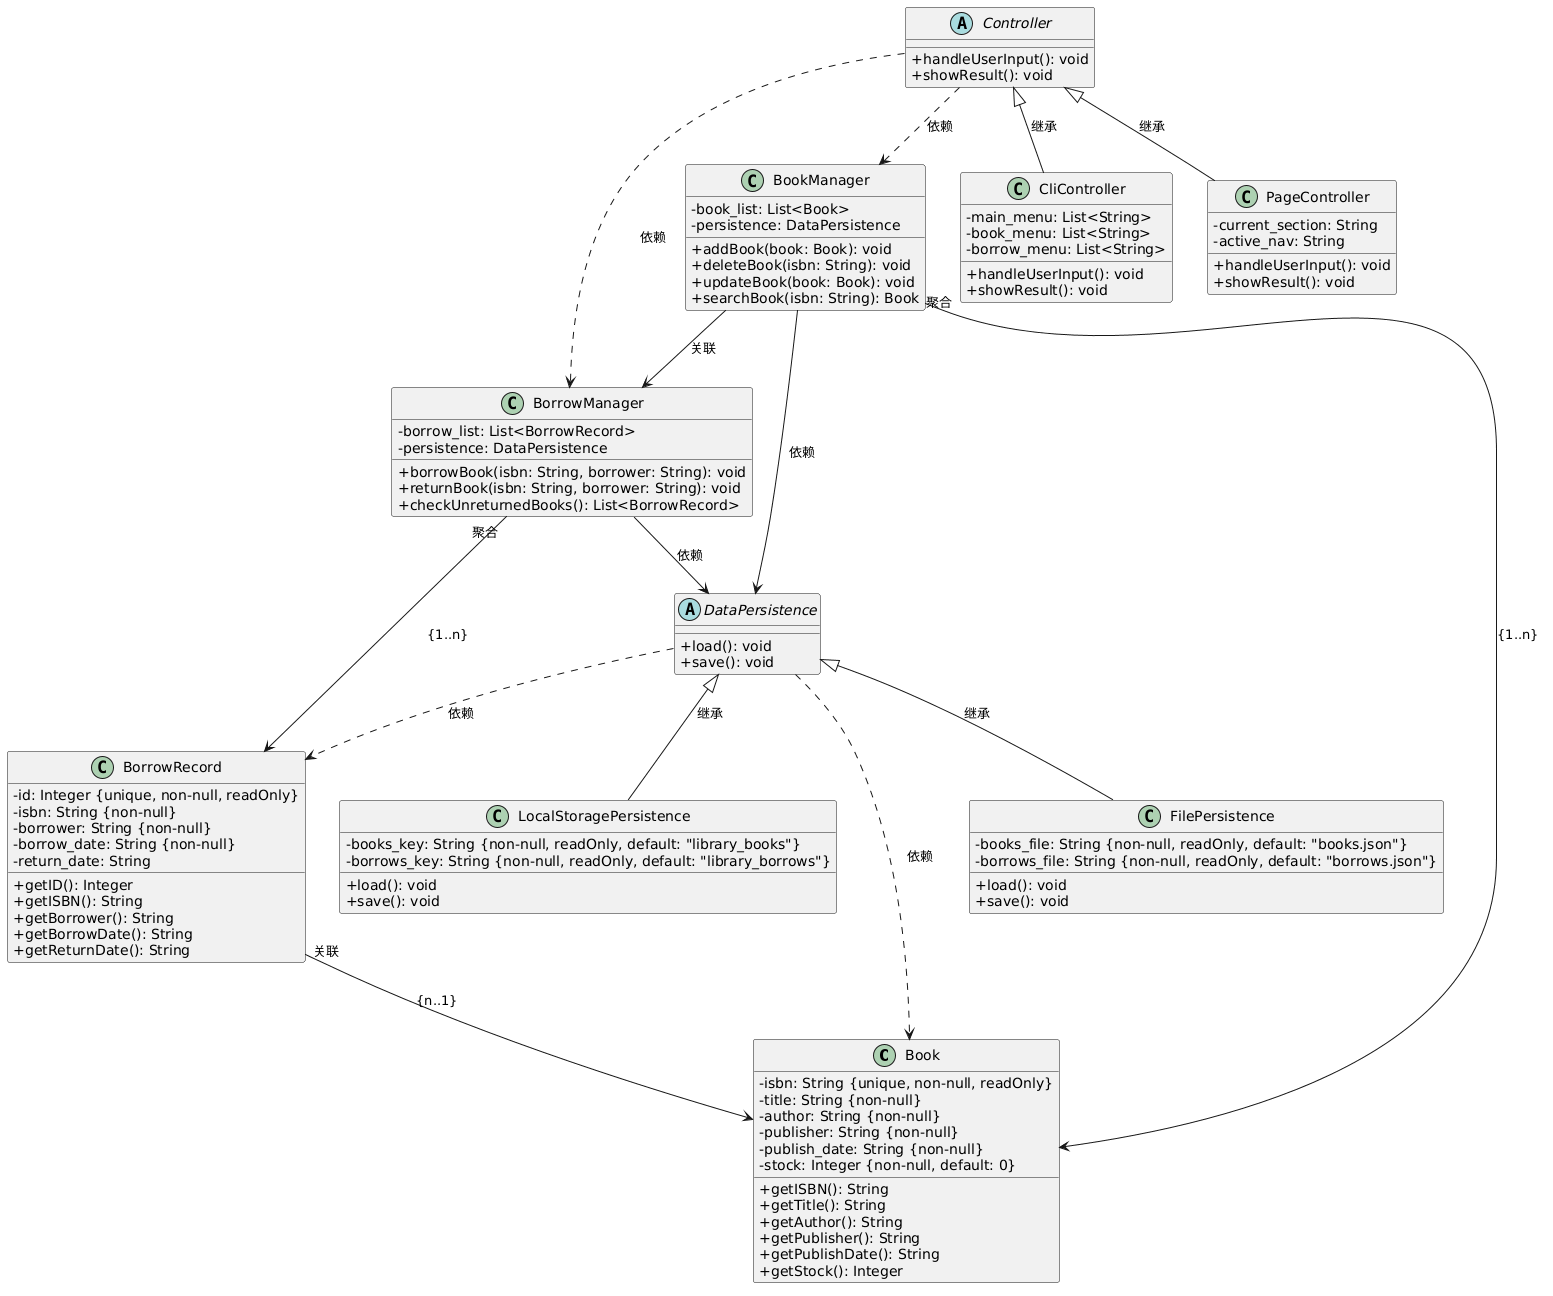
\includegraphics[width=0.8\textwidth]{DetailedClass.png}
    \caption{系统核心类总概述图}
    \label{fig:class_diagram}
\end{figure}



\subsection{实体类}

实体类为系统核心数据载体，位于实体层，无业务逻辑，仅封装属性与基础行为，被所有上层依赖。

\subsubsection{图书类}
\begin{verbatim}
from datetime import datetime
from typing import Optional

class Book:
    """图书实体类，封装图书核心属性与基础行为"""
    def __init__(
        self,
        id: str,
        isbn: str,
        book_name: str,
        author: str,
        publisher: Optional[str] = None,
        stock: int = 0,
        total_count: int = 0,
        create_time: Optional[datetime] = None,
        update_time: Optional[datetime] = None
    ):
        self.id = id  # 图书唯一ID，主键
        self.isbn = isbn  # 图书ISBN，唯一业务标识
        self.book_name = book_name  # 书名
        self.author = author  # 作者
        self.publisher = publisher  # 出版社
        self.stock = stock  # 可用库存
        self.total_count = total_count  # 总馆藏数量
        self.create_time = create_time or datetime.now()  # 入库时间
        self.update_time = update_time or datetime.now()  # 更新时间

    def is_available(self) -> bool:
        """判断图书是否可借阅"""
        return self.stock > 0

    def decrease_stock(self) -> bool:
        """扣减库存，借阅时调用"""
        if self.stock <= 0:
            return False
        self.stock -= 1
        self.update_time = datetime.now()
        return True

    def increase_stock(self) -> None:
        """增加库存，归还时调用"""
        self.stock += 1
        self.update_time = datetime.now()
\end{verbatim}
\subsubsection{借阅记录类}

\begin{verbatim}
from datetime import datetime
from typing import Optional

class BorrowRecord:
    """借阅记录实体类，封装借阅记录核心属性与基础行为"""
    def __init__(
        self,
        id: str,
        isbn: str,
        book_name: str,
        borrower_name: str,
        borrower_phone: Optional[str] = None,
        borrow_time: Optional[datetime] = None,
        return_time: Optional[datetime] = None,
        status: str = "未归还"
    ):
        self.id = id  # 借阅记录唯一ID，主键
        self.isbn = isbn  # 图书ISBN
        self.book_name = book_name  # 书名
        self.borrower_name = borrower_name  # 借阅人姓名
        self.borrower_phone = borrower_phone  # 借阅人联系电话
        self.borrow_time = borrow_time or datetime.now()  # 借阅时间
        self.return_time = return_time  # 归还时间
        self.status = status  # 借阅状态：未归还/已归还

    def is_unreturned(self) -> bool:
        """判断是否为未归还状态"""
        return self.status == "未归还"

    def complete_return(self) -> None:
        """完成归还操作，更新状态与归还时间"""
        self.status = "已归还"
        self.return_time = datetime.now()
\end{verbatim}

\subsubsection{用户类}
\begin{verbatim}
from datetime import datetime
from typing import Optional

class User:
    """用户实体类，封装系统用户核心属性"""
    def __init__(
        self,
        id: str,
        login_name: str,
        password: str,
        real_name: str,
        role: str,
        create_time: Optional[datetime] = None,
        update_time: Optional[datetime] = None
    ):
        self.id = id  # 用户唯一ID，主键
        self.login_name = login_name  # 登录用户名，唯一
        self.password = password  # 加密后的密码
        self.real_name = real_name  # 用户真实姓名
        self.role = role  # 用户角色：普通用户/图书管理员/系统维护人员
        self.create_time = create_time or datetime.now()  # 创建时间
        self.update_time = update_time or datetime.now()  # 更新时间

    def has_book_manage_permission(self) -> bool:
        """判断是否拥有图书管理权限"""
        return self.role == "图书管理员"

    def has_system_manage_permission(self) -> bool:
        """判断是否拥有系统管理权限"""
        return self.role == "系统维护人员"
\end{verbatim}

\subsection{数据访问类}

数据访问类位于数据访问层，封装本地存储/数据库的读写操作，屏蔽存储细节，为业务层提供统一的数据访问接口。

\subsubsection{基础DAO类}
\begin{verbatim}
from typing import List, Optional, TypeVar, Generic
import sqlite3

T = TypeVar('T')

class BaseDAO(Generic[T]):
    """基础DAO类，封装通用的CRUD操作，所有DAO类继承此类"""
    def __init__(self, db_path: str = "library.db"):
        self.db_path = db_path

    def _get_connection(self) -> sqlite3.Connection:
        """获取数据库连接"""
        return sqlite3.connect(self.db_path)

    def insert(self, entity: T) -> bool:
        """新增数据"""
        raise NotImplementedError("子类需实现insert方法")

    def update(self, entity: T) -> bool:
        """更新数据"""
        raise NotImplementedError("子类需实现update方法")

    def delete_by_id(self, id: str) -> bool:
        """根据ID删除数据"""
        raise NotImplementedError("子类需实现delete_by_id方法")

    def select_by_id(self, id: str) -> Optional[T]:
        """根据ID查询数据"""
        raise NotImplementedError("子类需实现select_by_id方法")

    def select_all(self) -> List[T]:
        """查询全量数据"""
        raise NotImplementedError("子类需实现select_all方法")
\end{verbatim}

\subsubsection{图书DAO类}

继承BaseDAO类，封装图书表的专属读写操作，包括按ISBN查询、多条件分页查询、库存更新等。

\subsubsection{借阅记录DAO类}

继承BaseDAO类，封装借阅记录表的专属读写操作，包括按ISBN查询未归还记录、按借阅人查询、按状态分页查询等。

\subsubsection{用户DAO类}

继承BaseDAO类，封装用户表的专属读写操作，包括按登录名查询用户、按角色查询用户等。

\subsection{规则校验类}

规则校验类位于规则校验层，封装系统通用业务规则与校验逻辑，实现规则复用，避免业务逻辑中重复编写校验代码。

\subsubsection{库存规则类}

\begin{verbatim}
from entities.Book import Book

class StockRule:
    """库存规则校验类，封装图书库存相关的所有校验规则"""

    @staticmethod
    def validate_borrow_stock(book: Book) -> tuple[bool, str]:
        """
        校验图书是否满足借阅库存条件
        :param book: 图书实体
        :return: (校验结果, 提示信息)
        """
        if not book:
            return False, "图书不存在"
        if not book.is_available():
            return False, "图书无可用库存，无法借阅"
        if book.stock < 0:
            return False, "图书库存异常，请联系管理员"
        return True, "校验通过"

    @staticmethod
    def validate_stock_number(stock: int, total_count: int) -> tuple[bool, str]:
        """
        校验库存数量合法性
        :param stock: 可用库存
        :param total_count: 总馆藏数量
        :return: (校验结果, 提示信息)
        """
        if stock < 0:
            return False, "可用库存不能为负数"
        if total_count < 0:
            return False, "总馆藏数量不能为负数"
        if stock > total_count:
            return False, "可用库存不能大于总馆藏数量"
        return True, "校验通过"
\end{verbatim}

\subsubsection{借阅规则类}

\begin{verbatim}
from entities.BorrowRecord import BorrowRecord

class BorrowRule:
    """借阅规则校验类，封装借阅/归还相关的所有校验规则"""

    @staticmethod
    def validate_return_record(record: BorrowRecord) -> tuple[bool, str]:
        """
        校验归还操作的借阅记录合法性
        :param record: 借阅记录实体
        :return: (校验结果, 提示信息)
        """
        if not record:
            return False, "借阅记录不存在"
        if not record.is_unreturned():
            return False, "该图书已完成归还，无需重复操作"
        return True, "校验通过"

    @staticmethod
    def validate_delete_book_has_unreturned(records: list[BorrowRecord]) -> tuple[bool, str]:
        """
        校验图书删除时是否存在未归还借阅记录
        :param records: 该图书的借阅记录列表
        :return: (校验结果, 提示信息)
        """
        for record in records:
            if record.is_unreturned():
                return False, "该图书存在未归还的借阅记录，无法删除"
        return True, "校验通过"
\end{verbatim}

\subsection{业务管理类}

业务管理类位于业务逻辑层，是核心业务规则的执行单元，封装对应模块的全量业务逻辑，编排业务流程，处理业务异常。

\subsubsection{图书管理器}

依赖BookDAO、StockRule、BorrowRule，封装图书管理全量业务逻辑，包括图书新增、查询、修改、删除的核心业务流程处理。

\subsubsection{借阅管理器}

依赖BorrowRecordDAO、BookDAO、BorrowRule、StockRule，封装借阅管理全量业务逻辑，包括图书借阅、归还、借阅记录查询的核心业务流程处理，事务控制。

\subsubsection{用户管理器}

依赖UserDAO，封装用户身份校验、权限加载、用户信息管理的核心业务逻辑。

\subsubsection{系统管理器}

依赖所有DAO类，封装系统数据备份、数据恢复、系统配置管理的核心业务逻辑。

\subsection{工具类}

工具类封装系统通用工具方法，实现代码复用，所有方法为静态方法，无状态，可全局调用。

\begin{enumerate}
\item  加密工具类（EncryptUtil）：封装密码加密、AES加解密、MD5摘要等方法

\item  验证码工具类（CaptchaUtil）：封装验证码生成、图片生成方法

\item  JWT工具类（JwtUtil）：封装Token生成、校验、解析方法

\item  日期工具类（DateUtil）：封装日期格式化、时间差计算等方法

\item  分页工具类（PageUtil）：封装分页参数处理、分页结果组装方法
\end{enumerate}

\section{页面详细设计}

\subsection{通用页面规范}

\begin{enumerate}
\item  页面布局：顶部导航栏+左侧菜单栏+主内容区的三段式布局，适配1920*1080及以上主流分辨率

\item  导航栏固定展示：系统名称、当前登录用户、角色、登出按钮

\item  菜单栏根据用户角色动态展示有权限的菜单，无权限的菜单隐藏

\item  所有表单提交前必须执行前端非空校验与格式校验，提交按钮点击后置灰，防止重复提交

\item  所有操作结果必须给出明确的成功/失败提示，异常场景给出可理解的错误信息
\end{enumerate}

\subsection{登录页面}

\subsubsection{页面入口}

系统根路径/，未登录用户访问任何页面均重定向至登录页

\subsubsection{页面元素}

\begin{enumerate}
\item  页面主体：系统logo、系统名称「图书管理系统」

\item  表单区域：

￮ 用户名输入框：placeholder「请输入用户名」

￮ 密码输入框：placeholder「请输入密码」，支持密码显隐切换

￮ 验证码输入框：placeholder「请输入验证码」，右侧展示验证码图片，点击图片可刷新

￮ 登录按钮：主按钮，点击提交登录请求

\item  底部版权信息
\end{enumerate}

\subsubsection{表单校验规则}

\begin{enumerate}
\item  用户名：非空校验，长度3-20位

\item  密码：非空校验，长度6-20位

\item  验证码：非空校验，长度4位

\item  任一校验不通过，登录按钮置灰，对应输入框下方给出红色提示文字
\end{enumerate}

\subsubsection{处理逻辑与后端交互}

\begin{enumerate}
\item  页面初始化完成后，前端生成32位随机imageCodeToken，调用验证码接口，渲染验证码图片

\item  验证码图片点击事件：重新生成imageCodeToken，调用验证码接口，刷新图片

\item  登录按钮点击事件：
\end{enumerate}

￮ 执行前端表单校验，校验不通过终止流程

￮ 对密码进行RSA前端加密，组装登录参数

￮ 调用登录接口

▪ 登录成功：前端存储Token与用户信息，根据角色跳转到对应首页，记录登录状态

▪ 登录失败：弹出错误提示，刷新验证码图片，清空验证码输入框，登录按钮恢复可点击状态

\subsection{首页}

\subsubsection{页面入口}

登录成功后默认跳转至/home，导航栏「首页」菜单

\subsubsection{页面元素与逻辑}

\begin{enumerate}
\item  系统欢迎语：展示当前登录用户姓名、角色

\item  系统功能介绍卡片：根据用户角色展示对应可操作的功能模块介绍与快捷入口

\item  数据概览区域：

￮ 普通用户：展示个人借阅总数、未归还数量、可借阅图书总数

￮ 图书管理员：展示馆藏图书总数、在借图书总数、可用库存总数、今日借阅/归还数量

￮ 系统维护人员：展示系统运行时长、数据备份次数、总用户数、总图书数

\item  快捷操作按钮：根据角色展示高频操作入口，如图书查询、借阅操作、新增图书等
\end{enumerate}

\subsection{图书管理页面}

\subsubsection{页面入口}

左侧菜单栏「图书管理」，仅图书管理员可访问，普通用户仅可访问图书查询子页面

\subsubsection{页面元素}

\begin{enumerate}
\item  查询区域：

￮ 查询类型下拉框：书名/作者/ISBN

￮ 关键词输入框：placeholder「请输入查询关键词」

￮ 查询按钮、重置按钮

\item  操作区域：图书管理员展示「新增图书」按钮

\item  图书列表表格：

￮ 列：ISBN、书名、作者、出版社、可用库存、总馆藏、入库时间、操作

￮ 操作列：图书管理员展示「修改」「删除」按钮，普通用户仅展示「查看详情」按钮

\item  分页组件：展示总条数、页码切换、每页条数调整

\item  新增/编辑弹窗：包含图书所有信息的表单，含表单校验

\item  删除确认弹窗：二次确认删除操作，提示风险
\end{enumerate}

\subsubsection{处理逻辑与后端交互}

\begin{enumerate}
\item  页面初始化：调用图书查询接口，加载第一页图书列表

\item  查询按钮点击事件：组装查询参数，调用图书查询接口，刷新列表

\item  新增按钮点击事件：打开新增弹窗，清空表单，用户填写后提交，调用图书新增接口，成功后关闭弹窗，刷新列表

\item  修改按钮点击事件：打开编辑弹窗，回显当前图书信息，用户修改后提交，调用图书修改接口，成功后关闭弹窗，刷新列表

\item  删除按钮点击事件：弹出二次确认弹窗，确认后调用图书删除接口，成功后刷新列表，失败弹出错误提示
\end{enumerate}

\subsection{借阅管理页面}

\subsubsection{页面入口}

左侧菜单栏「借阅管理」，所有登录用户可访问，根据角色展示不同功能

\subsubsection{页面元素}

\begin{enumerate}
\item  操作区域：「图书借阅」「图书归还」按钮

\item  查询区域：

￮ 查询类型下拉框：全部/个人借阅/未归还/按借阅人查询

￮ 借阅人输入框：仅查询类型为按借阅人查询时展示

￮ 查询按钮、重置按钮

\item  借阅记录列表表格：

￮ 列：记录ID、ISBN、书名、借阅人、借阅时间、归还时间、状态、操作

￮ 操作列：未归还状态展示「归还」按钮

\item  分页组件

\item  借阅操作弹窗：ISBN、借阅人信息表单

\item  归还操作弹窗：借阅记录ID、ISBN确认表单
\end{enumerate}

\subsubsection{处理逻辑与后端交互}

\begin{enumerate}
\item  页面初始化：根据用户角色调用借阅记录查询接口，加载对应列表

\item  借阅按钮点击事件：打开借阅弹窗，用户填写信息提交，调用图书借阅接口，成功后关闭弹窗，刷新列表与图书库存

\item  归还按钮点击事件：打开归还弹窗，回显借阅记录信息，用户确认后提交，调用图书归还接口，成功后关闭弹窗，刷新列表与图书库存

\item  查询按钮点击事件：组装查询参数，调用借阅记录查询接口，刷新列表
\end{enumerate}

\subsection{系统管理页面}

\subsubsection{页面入口}

左侧菜单栏「系统管理」，仅系统维护人员可访问

\subsubsection{页面元素}

\begin{enumerate}
\item  数据备份区域：「手动备份」按钮、备份记录列表、备份文件下载按钮

\item  数据恢复区域：备份文件上传组件、「开始恢复」按钮、恢复风险提示

\item  系统运行信息区域：展示系统版本、数据库大小、运行时长、备份记录统计
\end{enumerate}

\subsubsection{处理逻辑与后端交互}

\begin{enumerate}
\item  页面初始化：调用接口加载备份记录列表与系统运行信息

\item  手动备份按钮点击事件：调用数据备份接口，成功后刷新备份列表，提供文件下载

\item  恢复按钮点击事件：弹出二次确认弹窗，确认后上传备份文件，调用数据恢复接口，成功后提示用户重新登录
\end{enumerate}

\section{数据库设计}

\subsection{数据库选型}

基于需求文档「本地存储」要求，选型SQLite 3作为系统数据库，优势如下：
\begin{enumerate}
\item  轻量级嵌入式数据库，无需独立安装部署，单文件存储，适配全平台操作系统

\item  完全开源免费，无版权限制，符合项目经济可行性要求

\item  支持完整的关系型数据库特性，满足系统事务、索引、关联查询需求

\item  适配Python标准库，无需额外依赖，符合技术可行性要求
\end{enumerate}

\subsection{核心表结构设计}

\subsubsection{用户表}

\begin{table}[H]
    \centering
    \begin{tabular}{|l|l|l|l|l|l|}
        \hline
        字段名 & 类型 & 主键 & 非空 & 唯一 & 说明 \\
        \hline
        id & TEXT & 是 & 是 & 是 & 用户唯一ID，UUID生成 \\
        \hline
        login\_name & TEXT & 否 & 是 & 是 & 登录用户名 \\
        \hline
        password & TEXT & 否 & 是 & 否 & 加盐加密后的密码 \\
        \hline
        real\_name & TEXT & 否 & 是 & 否 & 用户真实姓名 \\
        \hline
        role & TEXT & 否 & 是 & 否 & 角色：用户/图书管理员/系统管理员\\
        \hline
        create\_time & DATETIME & 否 & 是 & 否 & 创建时间 \\
        \hline
        update\_time & DATETIME & 否 & 是 & 否 & 更新时间 \\
        \hline
    \end{tabular}
\end{table}
索引：login\_name  唯一索引

\subsubsection{图书表}

\begin{table}[H]
    \centering
    \begin{tabular}{|l|l|l|l|l|l|}
        \hline
        字段名 & 类型 & 主键 & 非空 & 唯一 & 说明 \\
        \hline
        id & TEXT & 是 & 是 & 是 & 图书唯一ID，UUID生成 \\
        \hline
        isbn & TEXT & 否 & 是 & 是 & 图书ISBN号，业务唯一标识 \\
        \hline
        book\_name & TEXT & 否 & 是 & 否 & 书名 \\
        \hline
        author & TEXT & 否 & 是 & 否 & 作者 \\
        \hline
        publisher & TEXT & 否 & 否 & 否 & 出版社 \\
        \hline
        stock & INTEGER & 否 & 是 & 否 & 可用库存，默认0，≥0 \\
        \hline
        total\_count & INTEGER & 否 & 是 & 否 & 总馆藏数量，默认0，≥0 \\
        \hline
        create\_time & DATETIME & 否 & 是 & 否 & 入库时间 \\
        \hline
        update\_time & DATETIME & 否 & 是 & 否 & 更新时间 \\
        \hline
    \end{tabular}
\end{table}

索引：isbn 唯一索引；book\_name 普通索引；author 普通索引

\subsubsection{借阅记录表}

\begin{table}[H]
    \centering
    \begin{tabular}{|l|l|l|l|l|l|}
        \hline
        字段名 & 类型 & 主键 & 非空 & 唯一 & 说明 \\
        \hline
        id & TEXT & 是 & 是 & 是 & 借阅记录唯一ID，UUID生成 \\
        \hline
        isbn & TEXT & 否 & 是 & 否 & 图书ISBN号 \\
        \hline
        book\_name & TEXT & 否 & 是 & 否 & 书名 \\
        \hline
        borrower\_name & TEXT & 否 & 是 & 否 & 借阅人姓名 \\
        \hline
        borrower\_phone & TEXT & 否 & 否 & 否 & 借阅人联系电话 \\
        \hline
        borrow\_time & DATETIME & 否 & 是 & 否 & 借阅时间 \\
        \hline
        return\_time & DATETIME & 否 & 否 & 否 & 归还时间，未归还为NULL \\
        \hline
        status & TEXT & 否 & 是 & 否 & 借阅状态：未归还/已归还，默认未归还 \\
        \hline
    \end{tabular}
\end{table}

索引：isbn 普通索引；borrower\_name 普通索引；status 普通索引

\subsubsection{系统配置表}

\begin{table}[H]
    \centering
    \begin{tabular}{|l|l|l|l|l|l|}
        \hline
        字段名 & 类型 & 主键 & 非空 & 唯一 & 说明 \\
        \hline
        id & TEXT & 是 & 是 & 是 & 配置ID \\
        \hline
        config\_key & TEXT & 否 & 是 & 是 & 配置键 \\
        \hline
        config\_value & TEXT & 否 & 是 & 否 & 配置值 \\
        \hline
        description & TEXT & 否 & 否 & 否 & 配置说明 \\
        \hline
        create\_time & DATETIME & 否 & 是 & 否 & 创建时间 \\
        \hline
        update\_time & DATETIME & 否 & 是 & 否 & 更新时间 \\
        \hline
    \end{tabular}
\end{table}

\subsubsection{操作日志表}

\begin{table}[H]
    \centering
    \begin{tabularx}{\linewidth}{|l|l|l|l|l|X|}
        \hline
        字段名 & 类型 & 主键 & 非空 & 唯一 & 说明 \\
        \hline
        id & TEXT & 是 & 是 & 是 & 日志ID \\
        \hline
        user\_id & TEXT & 否 & 是 & 否 & 操作人ID \\
        \hline
        user\_name & TEXT & 否 & 是 & 否 & 操作人姓名 \\
        \hline
        operation\_type & TEXT & 否 & 是 & 否 & 操作类型：登录/新增/修改/删除/借阅/归还/备份/恢复 \\
        \hline
        operation\_content & TEXT & 否 & 是 & 否 & 操作详情 \\
        \hline
        operation\_result & TEXT & 否 & 是 & 否 & 操作结果：成功/失败 \\
        \hline
        operation\_time & DATETIME & 否 & 是 & 否 & 操作时间 \\
        \hline
        ip\_address & TEXT & 否 & 否 & 否 & 操作IP地址 \\
        \hline
    \end{tabularx}
\end{table}

\subsection{数据库初始化脚本}

\begin{verbatim}
-- 创建用户表
CREATE TABLE IF NOT EXISTS sys_user (
    id TEXT PRIMARY KEY NOT NULL,
    login_name TEXT NOT NULL UNIQUE,
    password TEXT NOT NULL,
    real_name TEXT NOT NULL,
    role TEXT NOT NULL,
    create_time DATETIME NOT NULL DEFAULT (datetime('now', 'localtime')),
    update_time DATETIME NOT NULL DEFAULT (datetime('now', 'localtime'))
);

-- 创建图书表
CREATE TABLE IF NOT EXISTS book_info (
    id TEXT PRIMARY KEY NOT NULL,
    isbn TEXT NOT NULL UNIQUE,
    book_name TEXT NOT NULL,
    author TEXT NOT NULL,
    publisher TEXT,
    stock INTEGER NOT NULL DEFAULT 0 CHECK (stock >= 0),
    total_count INTEGER NOT NULL DEFAULT 0 CHECK (total_count >= 0),
    create_time DATETIME NOT NULL DEFAULT (datetime('now', 'localtime')),
    update_time DATETIME NOT NULL DEFAULT (datetime('now', 'localtime'))
);

-- 创建借阅记录表
CREATE TABLE IF NOT EXISTS borrow_record (
    id TEXT PRIMARY KEY NOT NULL,
    isbn TEXT NOT NULL,
    book_name TEXT NOT NULL,
    borrower_name TEXT NOT NULL,
    borrower_phone TEXT,
    borrow_time DATETIME NOT NULL DEFAULT (datetime('now', 'localtime')),
    return_time DATETIME,
    status TEXT NOT NULL DEFAULT '未归还' CHECK (status IN ('未归还', '已归还'))
);

-- 创建系统配置表
CREATE TABLE IF NOT EXISTS sys_config (
    id TEXT PRIMARY KEY NOT NULL,
    config_key TEXT NOT NULL UNIQUE,
    config_value TEXT NOT NULL,
    description TEXT,
    create_time DATETIME NOT NULL DEFAULT (datetime('now', 'localtime')),
    update_time DATETIME NOT NULL DEFAULT (datetime('now', 'localtime'))
);

-- 创建操作日志表
CREATE TABLE IF NOT EXISTS sys_operation_log (
    id TEXT PRIMARY KEY NOT NULL,
    user_id TEXT NOT NULL,
    user_name TEXT NOT NULL,
    operation_type TEXT NOT NULL,
    operation_content TEXT NOT NULL,
    operation_result TEXT NOT NULL,
    operation_time DATETIME NOT NULL DEFAULT (datetime('now', 'localtime')),
    ip_address TEXT
);

-- 创建索引
CREATE INDEX IF NOT EXISTS idx_book_isbn ON book_info(isbn);
CREATE INDEX IF NOT EXISTS idx_book_name ON book_info(book_name);
CREATE INDEX IF NOT EXISTS idx_book_author ON book_info(author);
CREATE INDEX IF NOT EXISTS idx_borrow_isbn ON borrow_record(isbn);
CREATE INDEX IF NOT EXISTS idx_borrower_name ON borrow_record(borrower_name);
CREATE INDEX IF NOT EXISTS idx_borrow_status ON borrow_record(status);
CREATE INDEX IF NOT EXISTS idx_user_login_name ON sys_user(login_name);

-- 初始化管理员用户（密码：admin123，已加密）
INSERT OR IGNORE INTO sys_user (id, login_name, password, real_name, role)
VALUES ('admin_001', 'admin', 'e10adc3949ba59abbe56e057f20f883e', '系统管理员', '系统维护人员');
\end{verbatim}

\section{工具与技术选型}

\subsection{开发语言与运行环境}

\begin{table}[H]
    \centering
    \begin{tabularx}{\linewidth}{|l|l|X|X|}
        \hline
        工具/环境 & 版本要求 & 选型说明 & 用途 \\
        \hline
        Python & 3.6及以上 & 需求文档指定技术栈，标准库即可实现核心功能，开源免费，跨平台兼容 & 系统核心开发语言 \\
        \hline
        SQLite & 3.30及以上 & 轻量级嵌入式数据库，单文件本地存储，无需独立部署，Python标准库原生支持 & 系统数据持久化存储 \\
        \hline
        Redis & 6.0及以上 & 开源内存数据库，高性能，支持过期时间设置，适配登录会话与验证码缓存 & 验证码、用户登录会话缓存 \\
        \hline
    \end{tabularx}
\end{table}

\subsection{核心框架与依赖库}

\begin{table}[H]
    \centering
    \begin{tabularx}{\linewidth}{|l|l|X|X|}
        \hline
        依赖库 & 版本要求 & 选型说明 & 用途 \\
        \hline
        FastAPI & 0.100.0+ & 轻量级高性能Python Web框架，自动生成接口文档，类型提示完善，开发效率高 & 后端Web服务框架，接口开发 \\
        \hline
        Uvicorn & 0.20.0+ & ASGI服务器，高性能，适配FastAPI，跨平台兼容 & Web服务部署运行 \\
        \hline
        Pydantic & 2.0.0+ & 数据校验库，与FastAPI无缝集成，实现入参出参类型校验 & 接口参数校验、DTO定义 \\
        \hline
        Passlib & 1.7.4+ & 密码加密库，支持多种加密算法，安全可靠 & 用户密码加密与校验 \\
        \hline
        Captcha & 0.4+ & 验证码生成库，轻量级，支持自定义验证码样式 & 图形验证码生成 \\
        \hline
        PyCryptodome & 3.18.0+ & 加密算法库，支持AES、RSA等主流加密算法 & 备份文件加解密、前端密码传输加密 \\
        \hline
        python-multipart & 0.0.6+ & 表单文件解析库，适配FastAPI文件上传 & 备份文件上传处理 \\
        \hline
    \end{tabularx}
\end{table}

\subsection{前端技术选型}

\begin{table}[H]
    \centering
    \begin{tabularx}{\linewidth}{|l|l|X|X|}
        \hline
        技术栈 & 版本要求 & 选型说明 & 用途 \\
        \hline
        Vue3 & 3.3.0+ & 渐进式JavaScript框架，组件化开发，上手简单，生态完善 & 前端页面开发 \\
        \hline
        Element Plus & 2.3.0+ & 适配Vue3的企业级UI组件库，样式统一，组件丰富 & 前端UI组件、表单、表格、弹窗等 \\
        \hline
        Axios & 1.4.0+ & HTTP请求库，支持请求/响应拦截，统一处理Token与异常 & 前端接口请求 \\
        \hline
        Vue Router & 4.2.0+ & Vue官方路由库，支持路由守卫，实现权限控制 & 前端页面路由管理 \\
        \hline
        Pinia & 2.1.0+ & Vue官方状态管理库，轻量级，支持持久化 & 前端全局状态管理（用户信息、Token） \\
        \hline
    \end{tabularx}
\end{table}

\subsection{开发与调试工具}

\begin{table}[H]
    \centering
    \begin{tabular}{|l|l|}
        \hline
        工具名称 & 用途 \\
        \hline
        PyCharm/VS Code & 后端Python代码开发与调试 \\
        \hline
        Visual Studio Code & 前端代码开发与调试 \\
        \hline
        Postman/Apifox & 接口调试与测试 \\
        \hline
        DB Browser for SQLite & SQLite数据库可视化管理 \\
        \hline
        Git & 代码版本管理 \\
        \hline
        PLantUML & 流程图、架构图、UML图绘制 \\
        \hline
    \end{tabular}
\end{table}

\newpage
\section{复用性设计}

减少重复代码，提升可维护性与可扩展性。

\subsection{代码级复用}

\begin{enumerate}
\item  通用工具类复用：将加密、验证码、日期、分页、数据库连接等通用逻辑封装为静态工具类，全局无状态调用，所有业务模块均可复用，避免重复实现。

\item  基础类继承复用：封装BaseDAO基础数据访问类，实现通用的CRUD方法，所有业务DAO类均继承此类，复用通用数据库操作逻辑，子类仅需实现专属业务方法。

\item  通用异常处理复用：封装全局统一异常处理器，定义系统自定义异常类，所有业务模块抛出的异常均由全局处理器统一处理，复用异常日志记录、响应格式封装逻辑。

\item  通用日志处理复用：封装统一的日志工具类，定义操作日志、安全日志、错误日志的规范，所有业务模块复用日志记录方法，保证日志格式统一。
\end{enumerate}

\subsection{组件级复用}

\begin{enumerate}
\item  前端通用组件复用：封装通用表单组件、表格组件、分页组件、弹窗组件、查询组件，所有业务页面均可复用，统一页面样式与交互逻辑，减少重复开发。

\item  权限控制组件复用：封装前端权限指令、后端登录拦截器、权限校验切面，所有接口与页面均复用权限控制逻辑，无需在每个业务中重复编写权限校验代码。

\item  参数校验组件复用：基于Pydantic封装通用参数校验基类，所有接口DTO均继承基类，复用通用非空校验、格式校验、类型校验逻辑。

\item  事务控制组件复用：封装数据库事务切面，所有需要事务控制的业务方法复用事务开启、提交、回滚逻辑，无需重复编写事务管理代码。
\end{enumerate}

\subsection{规则级复用}

\begin{enumerate}
\item  业务规则封装复用：将库存校验、借阅校验、ISBN唯一性校验等核心业务规则，封装为独立的规则校验类，所有涉及该规则的业务场景均可复用，保证业务规则的一致性。

\item  校验规则统一管理：将前端表单校验规则与后端接口校验规则统一管理，复用同一套校验逻辑，避免前后端校验规则不一致的问题。

\item  状态流转规则复用：封装图书状态、借阅记录状态的流转规则，所有涉及状态变更的业务均复用该规则，保证状态流转的规范性。
\end{enumerate}

\subsection{接口级复用}

\begin{enumerate}
\item  统一接口规范复用：所有接口遵循统一的请求路径、请求方式、响应格式、错误码规范，前端可复用统一的接口请求方法、响应处理逻辑、异常处理逻辑。

\item  通用接口复用：封装通用的分页查询接口、数据导出接口、字典查询接口，所有业务模块均可复用，无需重复开发同类接口。

\item  接口版本控制：采用/api/v1的路径版本控制方式，后续接口迭代可兼容旧版本接口，实现接口的向后兼容复用。
\end{enumerate}

\newpage
\section{跑批设计}

\subsection{数据自动备份跑批}

\subsubsection{基础信息}

\begin{enumerate}
\item  跑批名称：系统数据自动备份跑批

\item  执行周期：每日凌晨2:00执行一次

\item  触发方式：定时任务自动触发，支持手动触发

\item  执行环境：系统服务端，Python APScheduler定时任务框架
\end{enumerate}

\subsubsection{处理逻辑}

\begin{enumerate}
\item  定时任务触发后，先校验系统当前是否有活跃的业务操作，无操作则执行备份，有操作则延迟10分钟重试，最多重试3次

\item  读取数据库全量业务数据，生成JSON格式备份数据

\item  使用AES算法加密备份数据，生成以日期为命名的备份文件，保存至指定备份目录

\item  记录备份日志，包含备份时间、备份版本、文件大小、备份状态

\item  校验备份目录中的历史备份文件，仅保留最近30天的备份文件，超过30天的自动清理

\item  备份完成后，发送系统通知给系统维护人员，备份失败则发送告警通知
\end{enumerate}

\subsubsection{异常处理与重跑机制}

\begin{enumerate}
\item  备份过程中出现异常，立即记录异常日志，终止当前备份操作，不影响系统正常业务运行

\item  当日备份失败，系统将在凌晨3:00、4:00自动重试2次，3次均失败则停止重试，发送告警通知

\item  支持手动触发重跑，维护人员可在系统管理页面手动触发备份操作，补全当日备份
\end{enumerate}

\subsection{历史归档数据清理跑批}

\subsubsection{基础信息}

\begin{enumerate}
\item  跑批名称：历史归档数据清理跑批

\item  执行周期：每月1日凌晨3:00执行一次

\item  触发方式：定时任务自动触发

\item  执行环境：系统服务端，Python APScheduler定时任务框架
\end{enumerate}

\subsubsection{处理逻辑}

\begin{enumerate}
\item  定时任务触发后，查询1年以前的已完成归还的借阅记录，标记为归档数据

\item  将归档数据导出为备份文件，保存至归档目录，永久留存

\item  校验归档文件完整性，校验通过后，删除数据库中对应的归档借阅记录

\item  清理1年以前的操作日志数据，导出归档后删除数据库中对应数据

\item  记录清理日志，包含清理时间、清理数据量、归档文件信息

\item  清理完成后，执行数据库VACUUM操作，释放数据库存储空间，优化数据库性能
\end{enumerate}

\subsubsection{异常处理与重跑机制}

\begin{enumerate}
\item  清理过程中出现异常，立即回滚数据删除操作，记录异常日志，终止跑批

\item  支持手动触发重跑，维护人员可手动执行归档清理操作

\item  数据清理前必须完成全量数据备份，备份失败则终止清理操作
\end{enumerate}

\newpage
\section{安全设计}

\subsection{认证与授权安全}

\begin{enumerate}
\item  身份认证机制：基于Token的无状态认证机制，参考单点登录设计文档，用户登录成功后生成唯一Token，存入Redis设置2小时过期时间，超时自动登出。

\item  权限控制机制：基于RBAC角色权限模型，严格按照角色权限矩阵控制用户可访问的页面与接口，无权限请求直接拦截，前端隐藏无权限菜单与按钮。

\item  登录安全防护：所有登录操作均记录操作日志，包含登录IP、时间、结果
\end{enumerate}

\subsection{数据加密安全}

\begin{enumerate}
\item  传输加密：前端密码采用RSA非对称加密后传输，后端二次加盐加密，防止密码在传输过程中泄露。

\item  存储加密：备份文件采用AES对称加密存储，防止备份文件数据泄露；用户敏感信息加密存储，不存储明文敏感数据。

\item  加密算法规范：采用行业标准加密算法，密码加密使用MD5+盐值，非对称加密使用RSA2048，对称加密使用AES-128，不使用自定义不安全加密算法。
\end{enumerate}

\subsection{输入校验与防注入}

\begin{enumerate}
\item  全链路参数校验：前端表单校验+后端接口参数校验+数据库参数化查询，三层校验机制，防止非法参数传入。

\item  SQL注入防护：所有数据库查询均采用参数化查询，不拼接SQL语句，防止SQL注入攻击。

\item  XSS防护：所有前端输入的内容均进行转义处理，后端存储前进行特殊字符过滤，防止XSS跨站脚本攻击。

\item  CSRF防护：所有POST/PUT/DELETE请求均需携带Token，前端请求头统一携带，后端拦截器校验，防止CSRF跨站请求伪造攻击。
\end{enumerate}

\subsection{敏感数据处理}

\begin{enumerate}
\item  敏感数据脱敏：用户手机号、身份证号等敏感信息，前端展示时进行脱敏处理，仅展示部分字符。

\item  敏感操作审计：所有数据删除、数据恢复、用户管理等敏感操作，均记录详细的操作日志，包含操作人、操作时间、操作内容、操作IP、操作结果，可追溯可审计。

\item  数据访问控制：普通用户仅可访问个人相关数据，不可访问其他用户的借阅记录，图书管理员不可访问系统管理相关数据，严格控制数据访问边界。
\end{enumerate}

\subsection{业务安全规则}

\begin{enumerate}
\item  图书删除校验：存在未归还借阅记录的图书，禁止删除，防止数据丢失与业务异常。

\item  库存安全校验：库存扣减与恢复均在数据库事务中执行，防止超借、库存负数等异常情况。

\item  借阅记录不可篡改：借阅记录生成后，仅可更新归还时间与状态，不可修改借阅人、ISBN、借阅时间等核心信息，保证借阅记录的真实性与完整性。
\end{enumerate}

\newpage
\section{性能设计}

\subsection{查询性能优化}

\begin{enumerate}
\item  索引优化：为所有高频查询字段建立合适的索引，包括ISBN、书名、作者、借阅人、借阅状态、登录名等，避免全表扫描，提升查询效率。

\item  分页查询优化：所有列表查询均采用分页查询，限制每页最大条数，避免全量数据查询导致的内存占用过高与响应缓慢问题。

\item  关联查询优化：减少多表关联查询，借阅记录列表提前冗余书名信息，避免查询时关联图书表。

\item  缓存优化：高频访问的系统配置、图书分类数据，存入Redis缓存，减少数据库查询次数。
\end{enumerate}

\subsection{接口响应优化}

\begin{enumerate}
\item  接口超时控制：所有接口设置最大响应时间，慢查询接口记录告警日志，优化处理逻辑。

\item  非核心逻辑异步处理：操作日志记录、备份文件生成、通知发送等非核心逻辑，采用异步线程处理，不阻塞主业务流程，提升接口响应速度。

\item  数据压缩传输：接口响应数据采用Gzip压缩，减少网络传输数据量，提升前端加载速度。

\item  拦截器优化：登录校验、权限校验等拦截器逻辑采用Redis缓存查询，避免每次请求都查询数据库，减少接口处理耗时。
\end{enumerate}

\subsection{大数据量处理优化}

\begin{enumerate}
\item  数据归档清理：通过定时跑批，定期清理历史归档数据，控制单表数据量，避免单表数据量过大导致的查询性能下降。

\item  批量操作优化：批量新增图书等批量操作，采用批量写入数据库的方式，减少数据库IO次数，提升处理效率。

\item  流式处理：数据备份、数据导出等大数据量操作，采用流式读写方式，避免全量数据加载到内存导致的内存溢出问题。
\end{enumerate}

\subsection{存储性能优化}

\begin{enumerate}
\item  数据库定期优化：每月定时跑批执行数据库VACUUM操作，整理数据库文件碎片，释放存储空间，提升数据库读写性能。

\item  数据库连接优化：采用数据库连接池管理数据库连接，避免频繁创建与关闭数据库连接带来的性能开销。
\item  读写分离设计：预留读写分离扩展能力，查询操作走从库，写入操作走主库，为后续系统扩容提供支持。
\end{enumerate}

\newpage
\section{统一错误码设计}

系统采用统一的错误码规范，错误码为5位数字，前两位为模块编码，后三位为具体错误编码，便于问题定位与排查。

\begin{table}[H]
    \centering
    \begin{tabularx}{\linewidth}{|l|l|l|X|}
        \hline
        错误码 & 错误信息 & 模块 & 说明 \\
        \hline
        200 & 操作成功 & 通用 & 所有操作成功的统一响应码 \\
        \hline
        00001 & 参数校验失败 & 通用 & 入参格式、非空校验失败 \\
        \hline
        00002 & 系统内部异常 & 通用 & 服务器内部未知异常 \\
        \hline
        00003 & 无权限访问 & 通用 & 接口/页面无访问权限 \\
        \hline
        10001 & 验证码已过期 & 认证模块 & Redis中无对应验证码Token \\
        \hline
        10002 & 验证码错误 & 认证模块 & 验证码输入不匹配 \\
        \hline
        10003 & 用户名不存在或密码错误 & 认证模块 & 身份校验失败 \\
        \hline
        10004 & Token已过期或无效 & 认证模块 & 请求头Token无效/过期 \\
        \hline
        10005 & 账户已被锁定 & 认证模块 & 密码错误次数过多，账户锁定 \\
        \hline
        20001 & ISBN已存在 & 图书模块 & 新增图书时ISBN已存在 \\
        \hline
        20002 & 图书不存在 & 图书模块 & 图书ID/ISBN不存在 \\
        \hline
        20003 & 图书存在未归还借阅记录，无法删除 & 图书模块 & 删除图书时校验不通过 \\
        \hline
        20004 & 库存数量不合法 & 图书模块 & 库存/总馆藏为负数，或可用库存大于总馆藏 \\
        \hline
        30001 & 图书不存在 & 借阅模块 & 借阅/归还时ISBN对应的图书不存在 \\
        \hline
        30002 & 图书无可用库存，无法借阅 & 借阅模块 & 借阅时图书库存≤0 \\
        \hline
        30003 & 借阅记录不存在 & 借阅模块 & 归还时借阅记录ID不存在 \\
        \hline
        30004 & 该图书已归还，无需重复操作 & 借阅模块 & 归还时借阅记录已为已归还状态 \\
        \hline
        40001 & 备份文件非法，无法恢复 & 系统模块 & 数据恢复时备份文件校验失败 \\
        \hline
        40002 & 数据备份失败 & 系统模块 & 备份文件生成失败 \\
        \hline
        40003 & 数据恢复失败 & 系统模块 & 数据恢复执行失败 \\
        \hline
    \end{tabularx}
\end{table}

\newpage
\section{兼容性设计}

\subsection{操作系统兼容性}

1. 服务端兼容Windows 7/10/11、macOS、Linux全主流操作系统，无系统专属依赖，仅需Python环境即可运行。

2. 前端兼容Windows、macOS、Linux系统的主流浏览器，无操作系统专属限制。

\subsection{运行环境兼容性}

1. Python版本兼容Python 3.6及以上所有稳定版本，无低版本专属语法，核心功能可通过Python标准库实现。

2. SQLite兼容3.30及以上版本，采用通用SQL语法，无版本专属SQL语句。

3. 前端兼容Node.js 14.0及以上版本，适配Vue3的所有稳定运行环境。

\subsection{浏览器兼容性}

前端页面兼容以下主流浏览器的最新2个版本：

1. 谷歌浏览器（Chrome）

2. 火狐浏览器（Firefox）

3. Edge浏览器

4. Safari浏览器

5. 360浏览器、QQ浏览器等国产双核浏览器的极速模式

\subsection{分辨率兼容性}

1. 页面采用响应式布局，适配1366*768至4K的主流分辨率，保证页面元素正常展示，无错位、遮挡问题。

2. 表格、表单组件适配不同分辨率，支持横向滚动，保证小分辨率下可正常操作。

\section{测试要点设计}

\subsection{单元测试要点}

1. 实体类测试：测试实体类的核心方法，如库存扣减、状态更新、权限判断等方法的正确性。

2. 规则校验类测试：覆盖所有校验规则的正常场景与异常场景，测试校验结果的正确性。

3. 工具类测试：覆盖加密、验证码、日期、分页等工具类的所有方法，测试输出结果的正确性。

4. DAO类测试：测试数据库的增删改查操作，覆盖正常写入、异常场景、约束校验的正确性。

5. 业务Manager类测试：覆盖所有业务方法的正常流程、分支流程、异常流程，测试业务逻辑的正确性。

\subsection{集成测试要点}

1. 接口集成测试：覆盖所有接口的正常请求、参数异常、权限异常、业务异常场景，测试接口响应的正确性。

2. 数据库事务测试：测试借阅、归还、删除等涉及多表操作的事务回滚机制，异常场景下数据一致性。

3. 缓存集成测试：测试验证码、登录Token的缓存写入、读取、过期、删除逻辑的正确性。

4. 前后端交互测试：测试前端页面与后端接口的交互，参数传递、响应处理、异常提示的正确性。

5. 权限体系集成测试：测试不同角色用户的权限边界，无权限接口/页面的拦截机制是否生效。

\subsection{功能测试要点}

1. 登录功能测试：覆盖正常登录、用户名错误、密码错误、验证码过期、验证码错误、账户锁定、登出等场景。

2. 图书管理功能测试：覆盖图书新增、查询、修改、删除的所有正常与异常场景，ISBN唯一性校验、库存校验、删除约束校验。

3. 借阅管理功能测试：覆盖图书借阅、归还、借阅记录查询的所有场景，库存扣减与恢复、借阅状态更新、权限控制。

4. 系统管理功能测试：覆盖数据备份、数据恢复的正常与异常场景，备份文件生成、数据恢复回滚机制。

5. 页面交互测试：测试所有页面的渲染、表单校验、按钮操作、弹窗、分页、菜单权限显隐的正确性。

\subsection{性能测试要点}

1. 接口响应性能测试：测试核心接口的响应时间，单接口响应时间需≤200ms，并发100请求下无异常。

2. 大数据量查询性能测试：测试10万条图书/借阅记录下的分页查询性能，查询响应时间需≤500ms。

3. 并发操作测试：测试同一图书多用户同时借阅的并发场景，库存扣减正确性，无超借、脏数据问题。

4. 内存占用测试：测试系统长时间运行下的内存占用情况，无内存泄漏问题。

\subsection{安全测试要点}

1. SQL注入测试：测试所有接口的入参，传入SQL注入语句，验证是否存在注入漏洞。

2. XSS攻击测试：测试所有输入框，传入XSS脚本，验证是否存在跨站脚本漏洞。

3. 权限绕过测试：测试无权限用户直接访问接口/页面，验证权限拦截机制是否生效。

4. 暴力破解测试：测试登录接口，验证验证码机制、账户锁定机制是否生效。

5. 敏感数据泄露测试：测试接口响应、页面展示，验证敏感数据是否脱敏，是否存在明文密码泄露。

\newpage
\section{部署与运维设计}

\subsection{部署方式}

系统采用前后端分离部署方式，支持Windows、macOS、Linux全平台部署，提供两种部署方案：

\subsubsection{一键部署方案（推荐）}

1. 提供一键部署脚本，Windows系统提供bat脚本，Linux/macOS系统提供shell脚本

2. 脚本自动检查Python环境，安装所需依赖库，初始化数据库，启动后端服务

3. 前端打包为静态文件，集成到后端服务中，启动后即可通过浏览器访问

4. 部署完成后，默认访问地址：http://127.0.0.1:8000

\subsubsection{分步部署方案}

1. 环境准备：安装Python 3.6+、Node.js 14+

2. 后端部署：

￮ 克隆代码，进入后端目录，执行pip install -r requirements.txt安装依赖

￮ 执行初始化脚本，生成数据库文件

￮ 执行uvicorn main:app --host 0.0.0.0 --port 8000启动后端服务

3. 前端部署：

￮ 进入前端目录，执行npm install安装依赖

￮ 执行npm run build打包前端静态文件

￮ 将打包后的dist目录部署到Nginx，配置反向代理到后端服务

4. 缓存服务部署：安装Redis，配置后端Redis连接地址与密码

\subsection{环境要求}

\begin{table}[H]
    \centering
    \begin{tabularx}{\linewidth}{|l|X|X|}
        \hline
        环境类型 & 最低配置 & 推荐配置 \\
        \hline
        处理器 & Intel Core i3 同等性能 & Intel Core i5 及以上同等性能 \\
        \hline
        内存 & 4GB & 8GB及以上 \\
        \hline
        硬盘 & 100MB可用存储空间 & 1GB及以上可用存储空间 \\
        \hline
        操作系统 & Windows 7/macOS 10.13/Linux Kernel 4.14 & Windows 10/11、macOS 12+、Linux Kernel 5.4+ \\
        \hline
        网络 & 本地局域网访问，无需公网 & 支持公网访问，带宽10Mbps及以上 \\
        \hline
    \end{tabularx}
\end{table}

\subsection{数据备份与恢复策略}

1. 自动备份：每日凌晨自动执行全量数据备份，保留最近30天的备份文件，备份文件加密存储。

2. 手动备份：系统维护人员可在系统管理页面随时手动触发全量数据备份，生成备份文件。

3. 备份文件存储：本地备份目录存储，同时支持手动导出备份文件到外部存储设备，双重保障。

4. 数据恢复：系统提供可视化恢复功能，选择备份文件即可一键恢复系统数据，恢复前自动备份当前数据，恢复失败可回滚。

5. 数据库定期维护：每月执行一次数据库优化操作，整理碎片，优化性能，执行前自动备份全量数据。

\subsection{日常运维要点}

1. 系统状态监控：监控系统服务运行状态、内存占用、CPU占用、数据库文件大小，异常时及时告警。

2. 日志管理：系统运行日志、操作日志、安全日志按日期分割存储，保留最近1年的日志文件，定期清理过期日志。

3. 定期安全检查：每月检查系统操作日志，排查异常登录、异常操作。

4. 版本更新：系统版本更新前，必须完成全量数据备份；更新后，执行功能测试，验证系统正常运行。

5. 故障应急处理：制定故障应急处理流程，系统出现故障时，先停止服务，备份当前数据，再进行故障排查与修复，修复完成后重启服务验证。

\end{document}

